% Options for packages loaded elsewhere
\PassOptionsToPackage{unicode}{hyperref}
\PassOptionsToPackage{hyphens}{url}
%
\documentclass[
  a4paper,
]{article}
\usepackage{amsmath,amssymb}
\usepackage{iftex}
\ifPDFTeX
  \usepackage[T1]{fontenc}
  \usepackage[utf8]{inputenc}
  \usepackage{textcomp} % provide euro and other symbols
\else % if luatex or xetex
  \usepackage{unicode-math} % this also loads fontspec
  \defaultfontfeatures{Scale=MatchLowercase}
  \defaultfontfeatures[\rmfamily]{Ligatures=TeX,Scale=1}
\fi
\usepackage{lmodern}
\ifPDFTeX\else
  % xetex/luatex font selection
\fi
% Use upquote if available, for straight quotes in verbatim environments
\IfFileExists{upquote.sty}{\usepackage{upquote}}{}
\IfFileExists{microtype.sty}{% use microtype if available
  \usepackage[]{microtype}
  \UseMicrotypeSet[protrusion]{basicmath} % disable protrusion for tt fonts
}{}
\makeatletter
\@ifundefined{KOMAClassName}{% if non-KOMA class
  \IfFileExists{parskip.sty}{%
    \usepackage{parskip}
  }{% else
    \setlength{\parindent}{0pt}
    \setlength{\parskip}{6pt plus 2pt minus 1pt}}
}{% if KOMA class
  \KOMAoptions{parskip=half}}
\makeatother
\usepackage{xcolor}
\usepackage[margin=1in]{geometry}
\usepackage{color}
\usepackage{fancyvrb}
\newcommand{\VerbBar}{|}
\newcommand{\VERB}{\Verb[commandchars=\\\{\}]}
\DefineVerbatimEnvironment{Highlighting}{Verbatim}{commandchars=\\\{\}}
% Add ',fontsize=\small' for more characters per line
\usepackage{framed}
\definecolor{shadecolor}{RGB}{248,248,248}
\newenvironment{Shaded}{\begin{snugshade}}{\end{snugshade}}
\newcommand{\AlertTok}[1]{\textcolor[rgb]{0.94,0.16,0.16}{#1}}
\newcommand{\AnnotationTok}[1]{\textcolor[rgb]{0.56,0.35,0.01}{\textbf{\textit{#1}}}}
\newcommand{\AttributeTok}[1]{\textcolor[rgb]{0.13,0.29,0.53}{#1}}
\newcommand{\BaseNTok}[1]{\textcolor[rgb]{0.00,0.00,0.81}{#1}}
\newcommand{\BuiltInTok}[1]{#1}
\newcommand{\CharTok}[1]{\textcolor[rgb]{0.31,0.60,0.02}{#1}}
\newcommand{\CommentTok}[1]{\textcolor[rgb]{0.56,0.35,0.01}{\textit{#1}}}
\newcommand{\CommentVarTok}[1]{\textcolor[rgb]{0.56,0.35,0.01}{\textbf{\textit{#1}}}}
\newcommand{\ConstantTok}[1]{\textcolor[rgb]{0.56,0.35,0.01}{#1}}
\newcommand{\ControlFlowTok}[1]{\textcolor[rgb]{0.13,0.29,0.53}{\textbf{#1}}}
\newcommand{\DataTypeTok}[1]{\textcolor[rgb]{0.13,0.29,0.53}{#1}}
\newcommand{\DecValTok}[1]{\textcolor[rgb]{0.00,0.00,0.81}{#1}}
\newcommand{\DocumentationTok}[1]{\textcolor[rgb]{0.56,0.35,0.01}{\textbf{\textit{#1}}}}
\newcommand{\ErrorTok}[1]{\textcolor[rgb]{0.64,0.00,0.00}{\textbf{#1}}}
\newcommand{\ExtensionTok}[1]{#1}
\newcommand{\FloatTok}[1]{\textcolor[rgb]{0.00,0.00,0.81}{#1}}
\newcommand{\FunctionTok}[1]{\textcolor[rgb]{0.13,0.29,0.53}{\textbf{#1}}}
\newcommand{\ImportTok}[1]{#1}
\newcommand{\InformationTok}[1]{\textcolor[rgb]{0.56,0.35,0.01}{\textbf{\textit{#1}}}}
\newcommand{\KeywordTok}[1]{\textcolor[rgb]{0.13,0.29,0.53}{\textbf{#1}}}
\newcommand{\NormalTok}[1]{#1}
\newcommand{\OperatorTok}[1]{\textcolor[rgb]{0.81,0.36,0.00}{\textbf{#1}}}
\newcommand{\OtherTok}[1]{\textcolor[rgb]{0.56,0.35,0.01}{#1}}
\newcommand{\PreprocessorTok}[1]{\textcolor[rgb]{0.56,0.35,0.01}{\textit{#1}}}
\newcommand{\RegionMarkerTok}[1]{#1}
\newcommand{\SpecialCharTok}[1]{\textcolor[rgb]{0.81,0.36,0.00}{\textbf{#1}}}
\newcommand{\SpecialStringTok}[1]{\textcolor[rgb]{0.31,0.60,0.02}{#1}}
\newcommand{\StringTok}[1]{\textcolor[rgb]{0.31,0.60,0.02}{#1}}
\newcommand{\VariableTok}[1]{\textcolor[rgb]{0.00,0.00,0.00}{#1}}
\newcommand{\VerbatimStringTok}[1]{\textcolor[rgb]{0.31,0.60,0.02}{#1}}
\newcommand{\WarningTok}[1]{\textcolor[rgb]{0.56,0.35,0.01}{\textbf{\textit{#1}}}}
\usepackage{graphicx}
\makeatletter
\def\maxwidth{\ifdim\Gin@nat@width>\linewidth\linewidth\else\Gin@nat@width\fi}
\def\maxheight{\ifdim\Gin@nat@height>\textheight\textheight\else\Gin@nat@height\fi}
\makeatother
% Scale images if necessary, so that they will not overflow the page
% margins by default, and it is still possible to overwrite the defaults
% using explicit options in \includegraphics[width, height, ...]{}
\setkeys{Gin}{width=\maxwidth,height=\maxheight,keepaspectratio}
% Set default figure placement to htbp
\makeatletter
\def\fps@figure{htbp}
\makeatother
\setlength{\emergencystretch}{3em} % prevent overfull lines
\providecommand{\tightlist}{%
  \setlength{\itemsep}{0pt}\setlength{\parskip}{0pt}}
\setcounter{secnumdepth}{-\maxdimen} % remove section numbering
\ifLuaTeX
  \usepackage{selnolig}  % disable illegal ligatures
\fi
\IfFileExists{bookmark.sty}{\usepackage{bookmark}}{\usepackage{hyperref}}
\IfFileExists{xurl.sty}{\usepackage{xurl}}{} % add URL line breaks if available
\urlstyle{same}
\hypersetup{
  pdftitle={assignment 3 (mini project)},
  hidelinks,
  pdfcreator={LaTeX via pandoc}}

\title{assignment 3 (mini project)}
\author{}
\date{\vspace{-2.5em}2024-04-25}

\begin{document}
\maketitle

\begin{Shaded}
\begin{Highlighting}[]
\CommentTok{\# install necessary libraries}
\CommentTok{\#install.packages("ggplot2")}
\CommentTok{\#install.packages("pracma")}
\end{Highlighting}
\end{Shaded}

\begin{Shaded}
\begin{Highlighting}[]
\CommentTok{\# load required libraries}
\FunctionTok{library}\NormalTok{(dplyr)}
\end{Highlighting}
\end{Shaded}

\begin{verbatim}
## 
## Attaching package: 'dplyr'
\end{verbatim}

\begin{verbatim}
## The following objects are masked from 'package:stats':
## 
##     filter, lag
\end{verbatim}

\begin{verbatim}
## The following objects are masked from 'package:base':
## 
##     intersect, setdiff, setequal, union
\end{verbatim}

\begin{Shaded}
\begin{Highlighting}[]
\FunctionTok{library}\NormalTok{(readr)}
\FunctionTok{library}\NormalTok{(syuzhet)}

\CommentTok{\# read the CSV file}
\NormalTok{df }\OtherTok{\textless{}{-}} \FunctionTok{read.csv}\NormalTok{(}\StringTok{"data.csv"}\NormalTok{)}
\end{Highlighting}
\end{Shaded}

\begin{Shaded}
\begin{Highlighting}[]
\CommentTok{\# print the first 3 rows}
\FunctionTok{head}\NormalTok{(df, }\DecValTok{3}\NormalTok{)}
\end{Highlighting}
\end{Shaded}

\begin{verbatim}
##   beer_ABV beer_beerId beer_brewerId              beer_name
## 1      5.0       47986         10325           Sausa Weizen
## 2      6.2       48213         10325               Red Moon
## 3      6.5       48215         10325 Black Horse Black Beer
##               beer_style review_appearance review_palette review_overall
## 1             Hefeweizen               2.5            2.0            1.5
## 2     English Strong Ale               3.0            2.5            3.0
## 3 Foreign / Export Stout               3.0            2.5            3.0
##   review_taste review_profileName review_aroma
## 1          1.5            stcules          1.5
## 2          3.0            stcules          3.0
## 3          3.0            stcules          3.0
##                                                                                                                                                                                                                                                                                                                                                                                                    review_text
## 1                                                                                                                                       A lot of foam. But a lot. In the smell some banana, and then lactic and tart. Not a good start. Quite dark orange in color, with a lively carbonation (now visible, under the foam). Again tending to lactic sourness. Same for the taste. With some yeast and banana.
## 2                                                           Dark red color, light beige foam, average. In the smell malt and caramel, not really light. Again malt and caramel in the taste, not bad in the end. Maybe a note of honey in teh back, and a light fruitiness. Average body. In the aftertaste a light bitterness, with the malt and red fruit. Nothing exceptional, but not bad, drinkable beer.
## 3 Almost totally black. Beige foam, quite compact, not bad. Light smell, just a bit of roast, and some hop. A bit too light. The taste is light oo, and drinkable, with some malt, roast, hints of coffee. Nothing exceptional, but after all drinkable and pleasant. Light to average body. In the aftertaste some dust, somr roast, hint of caramel, and a bit of bitterness. No defect, drinkable, not bad.
##   review_time
## 1  1234817823
## 2  1235915097
## 3  1235916604
\end{verbatim}

\begin{Shaded}
\begin{Highlighting}[]
\CommentTok{\# print the last 3 rows}
\FunctionTok{tail}\NormalTok{(df, }\DecValTok{3}\NormalTok{)}
\end{Highlighting}
\end{Shaded}

\begin{verbatim}
##      beer_ABV beer_beerId beer_brewerId   beer_name              beer_style
## 1609     10.5        3635            22 La Terrible Belgian Strong Dark Ale
## 1610     10.5        3635            22 La Terrible Belgian Strong Dark Ale
## 1611     10.5        3635            22 La Terrible Belgian Strong Dark Ale
##      review_appearance review_palette review_overall review_taste
## 1609               3.5            4.0            3.5          4.5
## 1610               4.0            4.0            4.5          4.5
## 1611               4.0            3.5            3.0          3.0
##      review_profileName review_aroma
## 1609             weazal          4.0
## 1610            GRG1313          4.5
## 1611         coldmeat23          4.0
##                                                                                                                                                                                                                                                                                                                                                                                                                                                                                                                                                                                                                                                                                                                                                                                                                                                                                                                                                                                          review_text
## 1609                                                                                                                                                                                                                                                                                                                                                                                                                                                                                                                                                                                                       S: Dark and rich. Primarily raisins and malt, with a nice, low-key sweetness - like bread pudding made with with raisins and brandy. T: Mmmm...mild coffee up front under dominating carbonation that turns prickly halfway through until it dissolves into a powerful, thick, sticky, slightly bitter molasses/coffee flavor. Finishes like a stout - with a similar complex bitterness.
## 1610                                                                                                                                                                                                                                                                                                                                                                                                                                                                                                                                                                               Pours very dark brown with orange tint. Big carmel/toffee nose. Big flavors; gigantic flavor of cooked fruit and apricots with black coffee and sweet malt. Finish is medium/short and stops this from being cloyingly sweet. Soda pop character but good. Layered flavors of sweet malt, figs, prunes, raisins and brown sugar but with hints of cola and with a Dr. Pepper flavored finish. Different but nice.
## 1611 GLASS: Snifter TEMP: Cellared @ approx 45 degrees Pours a super dark brown color, almost black. Almost two-fingers of tan foam of medium density form the head. Retention is pretty good. Lacing is sporadic and fairly sticky. Dark fruits and brown sugars hit me first. Light phenols. Nice yeastiness. Good spice notes. Not quite the big nose that I was expecting. Again, this one is pretty subdued, which is not what was expected. Good malty backbone, with a fairly big yeastiness coming over the top of it. Nice spice notes. Mild notes of figs and dark fruits. Light touch of brown sugar. Not very complex, but a tasty brew, nonetheless. Almost full-bodied. Most of my enjoyment was killed by the high level of carbonation. It really gets in the way of everything else. It's just all sharp and fizzy, in the mouth, and completely detracts from this beer. While the high abv is nicely masked, the carbonation really kills the enjoyment level of this one for me.
##      review_time
## 1609  1246942776
## 1610  1246936211
## 1611  1246541885
\end{verbatim}

\begin{Shaded}
\begin{Highlighting}[]
\CommentTok{\# print the dimensions of the dataframe}
\FunctionTok{dim}\NormalTok{(df)}
\end{Highlighting}
\end{Shaded}

\begin{verbatim}
## [1] 1611   13
\end{verbatim}

\begin{Shaded}
\begin{Highlighting}[]
\CommentTok{\# print column names}
\FunctionTok{names}\NormalTok{(df)}
\end{Highlighting}
\end{Shaded}

\begin{verbatim}
##  [1] "beer_ABV"           "beer_beerId"        "beer_brewerId"     
##  [4] "beer_name"          "beer_style"         "review_appearance" 
##  [7] "review_palette"     "review_overall"     "review_taste"      
## [10] "review_profileName" "review_aroma"       "review_text"       
## [13] "review_time"
\end{verbatim}

\begin{Shaded}
\begin{Highlighting}[]
\CommentTok{\# print summary statistics}
\FunctionTok{summary}\NormalTok{(df)}
\end{Highlighting}
\end{Shaded}

\begin{verbatim}
##     beer_ABV       beer_beerId    beer_brewerId    beer_name        
##  Min.   : 0.100   Min.   :  436   Min.   :   22   Length:1611       
##  1st Qu.: 3.500   1st Qu.:  436   1st Qu.:  163   Class :character  
##  Median : 5.500   Median :10784   Median : 1075   Mode  :character  
##  Mean   : 5.408   Mean   :16086   Mean   : 1017                     
##  3rd Qu.: 6.100   3rd Qu.:25414   3rd Qu.: 1075                     
##  Max.   :10.500   Max.   :76963   Max.   :12770                     
##  NA's   :31                                                         
##   beer_style        review_appearance review_palette  review_overall 
##  Length:1611        Min.   :1.000     Min.   :1.000   Min.   :1.000  
##  Class :character   1st Qu.:3.000     1st Qu.:2.500   1st Qu.:3.000  
##  Mode  :character   Median :3.500     Median :3.500   Median :4.000  
##                     Mean   :3.475     Mean   :3.273   Mean   :3.515  
##                     3rd Qu.:4.000     3rd Qu.:4.000   3rd Qu.:4.000  
##                     Max.   :5.000     Max.   :5.000   Max.   :5.000  
##                                                                      
##   review_taste   review_profileName  review_aroma   review_text       
##  Min.   :1.000   Length:1611        Min.   :1.000   Length:1611       
##  1st Qu.:3.000   Class :character   1st Qu.:2.500   Class :character  
##  Median :3.500   Mode  :character   Median :3.500   Mode  :character  
##  Mean   :3.351                      Mean   :3.352                     
##  3rd Qu.:4.000                      3rd Qu.:4.000                     
##  Max.   :5.000                      Max.   :5.000                     
##                                                                       
##   review_time       
##  Min.   :9.882e+08  
##  1st Qu.:1.204e+09  
##  Median :1.259e+09  
##  Mean   :1.237e+09  
##  3rd Qu.:1.292e+09  
##  Max.   :1.326e+09  
## 
\end{verbatim}

\begin{Shaded}
\begin{Highlighting}[]
\CommentTok{\# print structure of the dataframe}
\FunctionTok{str}\NormalTok{(df)}
\end{Highlighting}
\end{Shaded}

\begin{verbatim}
## 'data.frame':    1611 obs. of  13 variables:
##  $ beer_ABV          : num  5 6.2 6.5 5 7.7 4.7 4.7 4.7 4.7 4.7 ...
##  $ beer_beerId       : int  47986 48213 48215 47969 64883 52159 52159 52159 52159 52159 ...
##  $ beer_brewerId     : int  10325 10325 10325 10325 1075 1075 1075 1075 1075 1075 ...
##  $ beer_name         : chr  "Sausa Weizen" "Red Moon" "Black Horse Black Beer" "Sausa Pils" ...
##  $ beer_style        : chr  "Hefeweizen" "English Strong Ale" "Foreign / Export Stout" "German Pilsener" ...
##  $ review_appearance : num  2.5 3 3 3.5 4 3.5 3.5 3.5 3.5 5 ...
##  $ review_palette    : num  2 2.5 2.5 3 4.5 3.5 3.5 2.5 3 3.5 ...
##  $ review_overall    : num  1.5 3 3 3 4 3 3.5 3 4 4.5 ...
##  $ review_taste      : num  1.5 3 3 2.5 4 3 4 2 3.5 4 ...
##  $ review_profileName: chr  "stcules" "stcules" "stcules" "stcules" ...
##  $ review_aroma      : num  1.5 3 3 3 4.5 3.5 4 3.5 4 4 ...
##  $ review_text       : chr  "A lot of foam. But a lot. In the smell some banana, and then lactic and tart. Not a good start. Quite dark oran"| __truncated__ "Dark red color, light beige foam, average. In the smell malt and caramel, not really light. Again malt and cara"| __truncated__ "Almost totally black. Beige foam, quite compact, not bad. Light smell, just a bit of roast, and some hop. A bit"| __truncated__ "Golden yellow color. White, compact foam, quite creamy. Good appearance. Fresh smell, with good hop. Quite dry,"| __truncated__ ...
##  $ review_time       : int  1234817823 1235915097 1235916604 1234725145 1293735206 1325524659 1318991115 1306276018 1290454503 1285632924 ...
\end{verbatim}

\begin{Shaded}
\begin{Highlighting}[]
\CommentTok{\# check unique cols in df}
\NormalTok{unique\_cols }\OtherTok{\textless{}{-}} \FunctionTok{sapply}\NormalTok{(df, }\ControlFlowTok{function}\NormalTok{(col) }\FunctionTok{length}\NormalTok{(}\FunctionTok{unique}\NormalTok{(col)) }\SpecialCharTok{==} \FunctionTok{length}\NormalTok{(col))}
\FunctionTok{print}\NormalTok{(}\FunctionTok{names}\NormalTok{(df)[unique\_cols])}
\end{Highlighting}
\end{Shaded}

\begin{verbatim}
## [1] "review_text" "review_time"
\end{verbatim}

\begin{Shaded}
\begin{Highlighting}[]
\CommentTok{\# check null counts}
\FunctionTok{colSums}\NormalTok{(}\FunctionTok{is.na}\NormalTok{(df))}
\end{Highlighting}
\end{Shaded}

\begin{verbatim}
##           beer_ABV        beer_beerId      beer_brewerId          beer_name 
##                 31                  0                  0                  0 
##         beer_style  review_appearance     review_palette     review_overall 
##                  0                  0                  0                  0 
##       review_taste review_profileName       review_aroma        review_text 
##                  0                  0                  0                  0 
##        review_time 
##                  0
\end{verbatim}

\begin{Shaded}
\begin{Highlighting}[]
\CommentTok{\# drop null values}
\NormalTok{df }\OtherTok{\textless{}{-}} \FunctionTok{na.omit}\NormalTok{(df)}
\FunctionTok{colSums}\NormalTok{(}\FunctionTok{is.na}\NormalTok{(df))}
\end{Highlighting}
\end{Shaded}

\begin{verbatim}
##           beer_ABV        beer_beerId      beer_brewerId          beer_name 
##                  0                  0                  0                  0 
##         beer_style  review_appearance     review_palette     review_overall 
##                  0                  0                  0                  0 
##       review_taste review_profileName       review_aroma        review_text 
##                  0                  0                  0                  0 
##        review_time 
##                  0
\end{verbatim}

\begin{Shaded}
\begin{Highlighting}[]
\CommentTok{\# print dimensions after dropping null values}
\FunctionTok{dim}\NormalTok{(df)}
\end{Highlighting}
\end{Shaded}

\begin{verbatim}
## [1] 1580   13
\end{verbatim}

\begin{Shaded}
\begin{Highlighting}[]
\FunctionTok{head}\NormalTok{(df}\SpecialCharTok{$}\NormalTok{review\_profileName)}
\end{Highlighting}
\end{Shaded}

\begin{verbatim}
## [1] "stcules"        "stcules"        "stcules"        "stcules"       
## [5] "johnmichaelsen" "oline73"
\end{verbatim}

\begin{Shaded}
\begin{Highlighting}[]
\CommentTok{\# sort by "review\_overall" in descending order}
\NormalTok{df }\OtherTok{\textless{}{-}}\NormalTok{ df }\SpecialCharTok{\%\textgreater{}\%} \FunctionTok{arrange}\NormalTok{(}\FunctionTok{desc}\NormalTok{(review\_overall))}
\CommentTok{\# keep the highest rating from each "review\_profileName" and drop the rest}
\NormalTok{df }\OtherTok{\textless{}{-}}\NormalTok{ df }\SpecialCharTok{\%\textgreater{}\%} \FunctionTok{distinct}\NormalTok{(review\_profileName, beer\_beerId, }\AttributeTok{.keep\_all =} \ConstantTok{TRUE}\NormalTok{)}
\CommentTok{\# print the dimensions of the dataframe}
\FunctionTok{dim}\NormalTok{(df)}
\end{Highlighting}
\end{Shaded}

\begin{verbatim}
## [1] 1574   13
\end{verbatim}

\begin{Shaded}
\begin{Highlighting}[]
\CommentTok{\# 1. Rank top 3 Breweries which produce the strongest beers?}

\CommentTok{\# group by brewerId and calculate the average ABV for each brewery}
\NormalTok{brewery\_avg\_abv }\OtherTok{\textless{}{-}}\NormalTok{ df }\SpecialCharTok{\%\textgreater{}\%}
\FunctionTok{group\_by}\NormalTok{(beer\_brewerId) }\SpecialCharTok{\%\textgreater{}\%}
\FunctionTok{summarize}\NormalTok{(}\AttributeTok{avg\_abv =} \FunctionTok{mean}\NormalTok{(beer\_ABV, }\AttributeTok{na.rm =} \ConstantTok{TRUE}\NormalTok{))}

\CommentTok{\# sort breweries by average ABV in descending order and select the top 3}
\NormalTok{top\_3\_breweries }\OtherTok{\textless{}{-}}\NormalTok{ brewery\_avg\_abv }\SpecialCharTok{\%\textgreater{}\%}
\FunctionTok{arrange}\NormalTok{(}\FunctionTok{desc}\NormalTok{(avg\_abv)) }\SpecialCharTok{\%\textgreater{}\%}
\FunctionTok{head}\NormalTok{(}\DecValTok{3}\NormalTok{)}

\CommentTok{\# print the top 3 breweries producing the strongest beers}
\FunctionTok{cat}\NormalTok{(}\StringTok{"Top 3 Breweries Producing the Strongest Beers:}\SpecialCharTok{\textbackslash{}n}\StringTok{"}\NormalTok{)}
\end{Highlighting}
\end{Shaded}

\begin{verbatim}
## Top 3 Breweries Producing the Strongest Beers:
\end{verbatim}

\begin{Shaded}
\begin{Highlighting}[]
\FunctionTok{print}\NormalTok{(top\_3\_breweries)}
\end{Highlighting}
\end{Shaded}

\begin{verbatim}
## # A tibble: 3 x 2
##   beer_brewerId avg_abv
##           <int>   <dbl>
## 1            22   10.5 
## 2           694   10.1 
## 3          2724    7.64
\end{verbatim}

\begin{Shaded}
\begin{Highlighting}[]
\CommentTok{\# 2. Which year did beers enjoy the highest ratings?}

\CommentTok{\# Convert review\_time to datetime}
\NormalTok{df}\SpecialCharTok{$}\NormalTok{review\_time }\OtherTok{\textless{}{-}} \FunctionTok{as.POSIXct}\NormalTok{(df}\SpecialCharTok{$}\NormalTok{review\_time, }\AttributeTok{origin =} \StringTok{"1970{-}01{-}01"}\NormalTok{, }\AttributeTok{tz =} \StringTok{"UTC"}\NormalTok{)}

\CommentTok{\# extract year from review\_time}
\NormalTok{df}\SpecialCharTok{$}\NormalTok{year }\OtherTok{\textless{}{-}} \FunctionTok{as.integer}\NormalTok{(}\FunctionTok{format}\NormalTok{(df}\SpecialCharTok{$}\NormalTok{review\_time, }\StringTok{"\%Y"}\NormalTok{))}

\CommentTok{\# group by year and calculate the average rating for each year}
\NormalTok{average\_ratings\_by\_year }\OtherTok{\textless{}{-}} \FunctionTok{aggregate}\NormalTok{(review\_overall }\SpecialCharTok{\textasciitilde{}}\NormalTok{ year, }\AttributeTok{data =}\NormalTok{ df, }\AttributeTok{FUN =}\NormalTok{ mean, }\AttributeTok{na.rm =} \ConstantTok{TRUE}\NormalTok{)}

\CommentTok{\# find the year with the highest average rating}
\NormalTok{highest\_rated\_year }\OtherTok{\textless{}{-}}\NormalTok{ average\_ratings\_by\_year[}\FunctionTok{which.max}\NormalTok{(average\_ratings\_by\_year}\SpecialCharTok{$}\NormalTok{review\_overall), }\StringTok{"year"}\NormalTok{]}

\FunctionTok{cat}\NormalTok{(}\StringTok{"Year with the highest average ratings for beers:"}\NormalTok{, highest\_rated\_year, }\StringTok{"}\SpecialCharTok{\textbackslash{}n}\StringTok{"}\NormalTok{)}
\end{Highlighting}
\end{Shaded}

\begin{verbatim}
## Year with the highest average ratings for beers: 2012
\end{verbatim}

\begin{Shaded}
\begin{Highlighting}[]
\CommentTok{\# 3. Based on the user’s ratings which factors are important among taste, aroma, appearance, and palette?}

\CommentTok{\# select columns for correlation calculation}
\NormalTok{correlation\_cols }\OtherTok{\textless{}{-}} \FunctionTok{c}\NormalTok{(}\StringTok{\textquotesingle{}review\_taste\textquotesingle{}}\NormalTok{, }\StringTok{\textquotesingle{}review\_aroma\textquotesingle{}}\NormalTok{, }\StringTok{\textquotesingle{}review\_appearance\textquotesingle{}}\NormalTok{, }\StringTok{\textquotesingle{}review\_palette\textquotesingle{}}\NormalTok{, }\StringTok{\textquotesingle{}review\_overall\textquotesingle{}}\NormalTok{)}
\NormalTok{correlation\_df }\OtherTok{\textless{}{-}}\NormalTok{ df[, correlation\_cols]}

\CommentTok{\# calculate correlation matrix}
\NormalTok{correlation\_matrix }\OtherTok{\textless{}{-}} \FunctionTok{cor}\NormalTok{(correlation\_df)}

\CommentTok{\# extract correlations with review\_overall}
\NormalTok{correlations\_with\_overall }\OtherTok{\textless{}{-}}\NormalTok{ correlation\_matrix[}\StringTok{\textquotesingle{}review\_overall\textquotesingle{}}\NormalTok{, ]}

\CommentTok{\# remove correlation with review\_overall}
\NormalTok{correlations\_with\_overall }\OtherTok{\textless{}{-}}\NormalTok{ correlations\_with\_overall[correlations\_with\_overall }\SpecialCharTok{!=} \DecValTok{1}\NormalTok{]}

\CommentTok{\# sort correlations in descending order}
\NormalTok{sorted\_correlations }\OtherTok{\textless{}{-}} \FunctionTok{sort}\NormalTok{(correlations\_with\_overall, }\AttributeTok{decreasing =} \ConstantTok{TRUE}\NormalTok{)}

\CommentTok{\# print correlations}
\FunctionTok{cat}\NormalTok{(}\StringTok{"Correlation between each factor and overall review rating:}\SpecialCharTok{\textbackslash{}n}\StringTok{"}\NormalTok{)}
\end{Highlighting}
\end{Shaded}

\begin{verbatim}
## Correlation between each factor and overall review rating:
\end{verbatim}

\begin{Shaded}
\begin{Highlighting}[]
\FunctionTok{print}\NormalTok{(sorted\_correlations)}
\end{Highlighting}
\end{Shaded}

\begin{verbatim}
##      review_aroma      review_taste    review_palette review_appearance 
##         0.8460822         0.7833555         0.7394945         0.6575341
\end{verbatim}

\begin{Shaded}
\begin{Highlighting}[]
\CommentTok{\# 4. If you were to recommend 3 beers to your friends based on this data which ones will you recommend?}

\CommentTok{\# define custom weights}
\NormalTok{weights }\OtherTok{\textless{}{-}} \FunctionTok{c}\NormalTok{(}\AttributeTok{review\_overall =} \FloatTok{0.4}\NormalTok{, }\AttributeTok{review\_taste =} \FloatTok{0.2}\NormalTok{, }\AttributeTok{review\_aroma =} \FloatTok{0.1}\NormalTok{, }\AttributeTok{review\_appearance =} \FloatTok{0.1}\NormalTok{, }\AttributeTok{review\_palette =} \FloatTok{0.2}\NormalTok{)}

\CommentTok{\# calculate weighted rating}
\NormalTok{df}\SpecialCharTok{$}\NormalTok{weighted\_rating }\OtherTok{\textless{}{-}} \FunctionTok{rowSums}\NormalTok{(df[, }\FunctionTok{names}\NormalTok{(weights)] }\SpecialCharTok{*}\NormalTok{ weights)}

\CommentTok{\# sort beers by weighted rating in descending order}
\NormalTok{recommended\_beers }\OtherTok{\textless{}{-}}\NormalTok{ df[}\FunctionTok{order}\NormalTok{(}\SpecialCharTok{{-}}\NormalTok{df}\SpecialCharTok{$}\NormalTok{weighted\_rating), ]}

\CommentTok{\# select top 3 recommended beers}
\NormalTok{recommended\_beers }\OtherTok{\textless{}{-}} \FunctionTok{head}\NormalTok{(recommended\_beers, }\DecValTok{3}\NormalTok{)}

\CommentTok{\# print recommended beers}
\FunctionTok{cat}\NormalTok{(}\StringTok{"Recommended beers for my friends:}\SpecialCharTok{\textbackslash{}n}\StringTok{"}\NormalTok{)}
\end{Highlighting}
\end{Shaded}

\begin{verbatim}
## Recommended beers for my friends:
\end{verbatim}

\begin{Shaded}
\begin{Highlighting}[]
\FunctionTok{print}\NormalTok{(recommended\_beers[, }\FunctionTok{c}\NormalTok{(}\StringTok{"beer\_name"}\NormalTok{, }\StringTok{"weighted\_rating"}\NormalTok{)])}
\end{Highlighting}
\end{Shaded}

\begin{verbatim}
##             beer_name weighted_rating
## 27        Caldera IPA            5.00
## 55 T.J.'s Best Bitter            5.00
## 38              Mogli            4.95
\end{verbatim}

\begin{Shaded}
\begin{Highlighting}[]
\CommentTok{\# 5. Which Beer style seems to be the favorite based on reviews written by users?}
\CommentTok{\# 6. How does written review compare to overall review score for the beer styles? (together)}

\CommentTok{\# select relevant columns}
\NormalTok{reviewTextData }\OtherTok{\textless{}{-}}\NormalTok{ df[, }\FunctionTok{c}\NormalTok{(}\StringTok{\textquotesingle{}beer\_beerId\textquotesingle{}}\NormalTok{, }\StringTok{\textquotesingle{}beer\_name\textquotesingle{}}\NormalTok{, }\StringTok{\textquotesingle{}beer\_ABV\textquotesingle{}}\NormalTok{, }\StringTok{\textquotesingle{}beer\_style\textquotesingle{}}\NormalTok{, }\StringTok{\textquotesingle{}review\_overall\textquotesingle{}}\NormalTok{, }\StringTok{\textquotesingle{}review\_text\textquotesingle{}}\NormalTok{)]}

\CommentTok{\# filter rows with review\_overall \textgreater{}= 4}
\NormalTok{reviewTextData }\OtherTok{\textless{}{-}}\NormalTok{ reviewTextData[reviewTextData}\SpecialCharTok{$}\NormalTok{review\_overall }\SpecialCharTok{\textgreater{}=} \DecValTok{4}\NormalTok{, ]}

\CommentTok{\# reset index}
\FunctionTok{rownames}\NormalTok{(reviewTextData) }\OtherTok{\textless{}{-}} \ConstantTok{NULL}

\CommentTok{\# print the first few rows}
\FunctionTok{print}\NormalTok{(}\FunctionTok{head}\NormalTok{(reviewTextData))}
\end{Highlighting}
\end{Shaded}

\begin{verbatim}
##   beer_beerId           beer_name beer_ABV              beer_style
## 1       52159 Caldera Ginger Beer      4.7    Herbed / Spiced Beer
## 2       58046       Rauch Ür Bock      7.4               Rauchbier
## 3       58046       Rauch Ür Bock      7.4               Rauchbier
## 4       58046       Rauch Ür Bock      7.4               Rauchbier
## 5       25414    Caldera Pale Ale      5.5 American Pale Ale (APA)
## 6       25414    Caldera Pale Ale      5.5 American Pale Ale (APA)
##   review_overall
## 1              5
## 2              5
## 3              5
## 4              5
## 5              5
## 6              5
##                                                                                                                                                                                                                                                                                                                                                                                                                                                                                                                                                                                                                                                                                                                                                                                                                                                                                                                                                                                                                                                                                                                                                                                                                                                                                                                                                                                                                                                                                                                                                                                                                                                                                                                                                                                                                                                                                                                                                                                                                                                                                                                                             review_text
## 1 OK, so the only reason I bought this while shopping at Whole Foods was because I've never had a "ginger beer" unless it was ginger ALE...and we all know that's not the kind of "beer" we're interested in on this site! I was very excited to try this one!... When poured out it looks like a cheapo macro lager at first sight, then the slowly fading head suggests otherwise. The body is crystal clear and is a very light straw color. The head is bright white and slowly dissipates, but is initially quite thick. Smell is adjuncty, but there are slight notes of honey and some kind of herby thing going on...ginger perhaps? Can't really tell. From the smell there is obviously something different about this beer though. It has a unique spicy smell to it and reminds me a lot of basil, not ginger. I really can't quite place everything that I smell, but it is a very nice aroma. Superb fragrance for this beer, though definitely not a "ginger beer" based on the smell. The taste is very unique also. It's kind of like a spiced pilsner or kolsch but the "spice" is kind of hard to identify. It does not taste like ginger. This beer actually reminds me a lot of Bison's Honey Basil ale. There is some definite astringent burn in the upper throat after swallowing that is no doubt from the ginger, but that is the only ginger I can detect with any certainty. It is only slightly hoppy and malty. This a very enjoyable, very drinkable beer (I could easily drink 2 22oz'ers) but I think it's failing in its claim to be a "ginger" beer because I don't smell it, can barely taste it, and can only really detect the ginger's physiological effects of a warm throat and stomach. So, rating this one is hard; I've never had a ginger beer so I don't really know what one ought to taste like...but then again I can't really tell if I'm tasting ginger here or the combination of other things. So confused. My recommendation to you Caldera folks: ADD MORE GINGER! There's obviously enough of a curiosity about this style to not hurt sales if it was strengthened. I for one could handle it.
## 2                                                                                                                                                                                                                                                                                                                                                                                                                                                                                                                                                                                                                                                                                                                                                                                                                                                                                                                                                                                                                                                                                                                                                                                                                                                                                                                                                                                                                                                                                                                                                                                                                         Pours a mahogany color, rich, with a tan head. a finger, didn't stick around. Holy smokes! This is one of the most smokiest beer I've ever had! BUT. It's balance and not one sided. Smoke, cured bacon, rich caramel malts. More smoke. Ok, maybe it one sided, but it's heavenly. Rich caramel malts and salty cured bacon strips. Bacon lover right here, so, I don't feel the need to go on. Lighter, but medium in body. feels fine. Nothing tremendous. Aroma and flavor alone are mouthwatering. Bravo. More please!!!
## 3                                                                                                                                                                                                                                                                                                                                                                                                                                                                                                                                                                                                                                                                                                                                                                                                                                                                                                                                                                                                                                                                                                                                                                                                                                                                                                       22 oz. Think I picked this up in Chicago Binny's Oak Park. Solid amber/brown pour, half finger of off white head disappated to a ring, but lasted. Smoked malt, peat, canadian bacon and some malty caramel. Starting out real well. Taste, solid dose of smoked ham, bacon, peat and a woodiness. Caramelly malt body is there, almost some faint raisin or apple cider, then finishes with solid bbq. The real deal, far far and away the best American version I've had of this style. So few try this style, even less accomplish the task. Lighter side of medium bodied. Coats well, goes down smooth, no alcohol. 7.4 is a little larger than some for the style, but it doesn't show itself. Best brew I've had in a while. First I've had from this brewery, if their others are even close to as good as this I won't be disapointed.
## 4                                                                                                                                                                                                                                                                                                                                                                                                                                                                                                                                                                                                                                                                                                                                                                                                                                                                                                                                                                                                                                                                                                                                                                    A-Bright, crystal clear, copper with a medium tan head that slowly fades to a thin cap and leaves light lace. S-Campfire smoke with a subtle hit of applewoods smoked bacon. Sweet caramel malt and spicy pepper notes accent in the background. T-Yes, this is a smoked brew but it never comes off as over the top. In fact it is about as perfect as it can get. Dry, woody smokiness and spicy, herbal hops dominate. Caramel malt sweetness provides a healthy backbone with tones of toasted biscuit, apple and buckwheat honey. M-Medium bodied with a feel that is bigger than it really is. Smooth and slick with a drying, woody astringency in the finish. Nice lingering sweet smokiness. D-Simply put---&gt;OUTSTANDING! Quite possibly one of the finest Rauch beers I have had the pleasure of imbibing! This is a beer I wish I would have tried sooner so I could have gone out and stocked up on. Well done Caldera, this is a beer you should be VERY proud of!
## 5                                                                                                                                                                                                                                                                                                                                                                                                                                                                                                                                                                                                                                                                                                                                                                                                                                                                                   I'm really enjoying the variety of quality brews in a CAN i'm finding here in Northern California! this was reviewed while camping at Castle lake campgrounds in shasta city...i think. Ooooh yeah, cracking open a can sounds good!! a thick, solid and rocky -white head stands proud like Mt. shasta itself over a bright plae golden liquid, much like the N.Cali sunsets. Retention is amazing, it's not going anywhere anytime soon. The nose is just bursting with hoppy cascade aroma's!! Sweet fruits, musty herbs, wheat and corn and light but sweet malt. This all cascade beauty has a great aroma. The hoppy flavor's here are deep and very complex, cascade hoppiness all in my face. Light and very, very crispy feel is exciting and spot-on for the style. crisp with a creamy smooth finish from the beastie foam still clumping it's way down slow. The cascade hops provide a gentle fruitiness and perfect dry-herbal and earthy complexity. I havn't been this excited for a Pale ale since my very first Sierra Nevada!!(circa 1996) This pale ale in a can has made my day, and I'm camping in one of the most pristine locations I've ever been too. This is simply one of, if not THE best Pale ale i've ever had. Bring on the cans!!!
## 6                                                                                                                                                                                                                                                                                                                                                                                                                                                                                                                                                                                                                                                                                                                                                                                                                                                                                                                                                                                                                                                                                                                                                                                                                                                                                                                                                                                                                               Poured from a can into a pint glass. A: Pours clear, golden color with a one-finger off-white head that quickly leaves. S: Aroma is light & simple, floral citrus hops with some caramel malts lingering on the tale end. T: More than expected from the aroma. Lots of citrus flavors, grapefruit, lemon, orange & a bit of toasted malt. Very clean & tasty! Can't wait for another sip! M: Medium-full, kind of oily, moving to a crisp off-dry some what spicy finish. D: Fantastic drinkability! A huge fan of what Caldera is doing with cans. Awesome for camping/hiking, skiing, fishing, or anything where you don't want the weight of a bottle, but the quality of a micro brew. Easy to pack-in & pack-out.
\end{verbatim}

\begin{Shaded}
\begin{Highlighting}[]
\NormalTok{reviewTextData}\SpecialCharTok{$}\NormalTok{review\_text[}\DecValTok{8}\NormalTok{]}
\end{Highlighting}
\end{Shaded}

\begin{verbatim}
## [1] "Clear golden-orange color with small white head that laces well. Slightly sweet and spicy toasty grain with some floral and slightly woodsy and fruity hops. Lightly toasted and sweet fruity pale malts perfectly balanced by orangey citrus and floral hop bitterness that's a bit persistent. Nice light-moderate body that feels even easier due to the high, but no too stingy carbonation. Extremely drinkable Pale that I would definitely buy again."
\end{verbatim}

\begin{Shaded}
\begin{Highlighting}[]
\CommentTok{\# text preprocessing: replacing contractions with their full forms}
\NormalTok{decontracted }\OtherTok{\textless{}{-}} \ControlFlowTok{function}\NormalTok{(phrase) \{}
  \CommentTok{\# Specific contractions}
\NormalTok{  phrase }\OtherTok{\textless{}{-}} \FunctionTok{gsub}\NormalTok{(}\StringTok{"won\textquotesingle{}t"}\NormalTok{, }\StringTok{"will not"}\NormalTok{, phrase)}
\NormalTok{  phrase }\OtherTok{\textless{}{-}} \FunctionTok{gsub}\NormalTok{(}\StringTok{"can\textquotesingle{}t"}\NormalTok{, }\StringTok{"can not"}\NormalTok{, phrase)}
\NormalTok{  phrase }\OtherTok{\textless{}{-}} \FunctionTok{gsub}\NormalTok{(}\StringTok{"it\textquotesingle{}s"}\NormalTok{, }\StringTok{"it is"}\NormalTok{, phrase)}
  
  \CommentTok{\# general contractions}
\NormalTok{  phrase }\OtherTok{\textless{}{-}} \FunctionTok{gsub}\NormalTok{(}\StringTok{"n\textquotesingle{}t"}\NormalTok{, }\StringTok{" not"}\NormalTok{, phrase)}
\NormalTok{  phrase }\OtherTok{\textless{}{-}} \FunctionTok{gsub}\NormalTok{(}\StringTok{"\textquotesingle{}re"}\NormalTok{, }\StringTok{" are"}\NormalTok{, phrase)}
\NormalTok{  phrase }\OtherTok{\textless{}{-}} \FunctionTok{gsub}\NormalTok{(}\StringTok{"\textquotesingle{}s"}\NormalTok{, }\StringTok{" is"}\NormalTok{, phrase)}
\NormalTok{  phrase }\OtherTok{\textless{}{-}} \FunctionTok{gsub}\NormalTok{(}\StringTok{"\textquotesingle{}d"}\NormalTok{, }\StringTok{" would"}\NormalTok{, phrase)}
\NormalTok{  phrase }\OtherTok{\textless{}{-}} \FunctionTok{gsub}\NormalTok{(}\StringTok{"\textquotesingle{}ll"}\NormalTok{, }\StringTok{" will"}\NormalTok{, phrase)}
\NormalTok{  phrase }\OtherTok{\textless{}{-}} \FunctionTok{gsub}\NormalTok{(}\StringTok{"\textquotesingle{}t"}\NormalTok{, }\StringTok{" not"}\NormalTok{, phrase)}
\NormalTok{  phrase }\OtherTok{\textless{}{-}} \FunctionTok{gsub}\NormalTok{(}\StringTok{"\textquotesingle{}ve"}\NormalTok{, }\StringTok{" have"}\NormalTok{, phrase)}
\NormalTok{  phrase }\OtherTok{\textless{}{-}} \FunctionTok{gsub}\NormalTok{(}\StringTok{"\textquotesingle{}m"}\NormalTok{, }\StringTok{" am"}\NormalTok{, phrase)}
  
  \FunctionTok{return}\NormalTok{(phrase)}
\NormalTok{\}}
\end{Highlighting}
\end{Shaded}

\begin{Shaded}
\begin{Highlighting}[]
\CommentTok{\# define an empty list to store preprocessed reviews}
\NormalTok{preprocessed\_reviews }\OtherTok{\textless{}{-}} \FunctionTok{c}\NormalTok{()}

\CommentTok{\# loop through each review text}
\ControlFlowTok{for}\NormalTok{ (sentence }\ControlFlowTok{in}\NormalTok{ reviewTextData}\SpecialCharTok{$}\NormalTok{review\_text) \{}
\NormalTok{  sentence }\OtherTok{\textless{}{-}} \FunctionTok{decontracted}\NormalTok{(sentence)}
  
  \CommentTok{\# remove words with numbers}
\NormalTok{  sentence }\OtherTok{\textless{}{-}} \FunctionTok{gsub}\NormalTok{(}\StringTok{"}\SpecialCharTok{\textbackslash{}\textbackslash{}}\StringTok{S*}\SpecialCharTok{\textbackslash{}\textbackslash{}}\StringTok{d}\SpecialCharTok{\textbackslash{}\textbackslash{}}\StringTok{S*"}\NormalTok{, }\StringTok{""}\NormalTok{, sentence)}
  
\NormalTok{  sentence }\OtherTok{\textless{}{-}} \FunctionTok{trimws}\NormalTok{(sentence)}
\NormalTok{  preprocessed\_reviews }\OtherTok{\textless{}{-}} \FunctionTok{c}\NormalTok{(preprocessed\_reviews, sentence)}
\NormalTok{\}}

\NormalTok{preprocessed\_reviews[}\DecValTok{8}\NormalTok{] }\CommentTok{\# check how that\textquotesingle{}s changed to that is}
\end{Highlighting}
\end{Shaded}

\begin{verbatim}
## [1] "Clear golden-orange color with small white head that laces well. Slightly sweet and spicy toasty grain with some floral and slightly woodsy and fruity hops. Lightly toasted and sweet fruity pale malts perfectly balanced by orangey citrus and floral hop bitterness that is a bit persistent. Nice light-moderate body that feels even easier due to the high, but no too stingy carbonation. Extremely drinkable Pale that I would definitely buy again."
\end{verbatim}

\begin{Shaded}
\begin{Highlighting}[]
\CommentTok{\# append preprocessed reviews to the filtered dataframe}
\NormalTok{reviewTextData}\SpecialCharTok{$}\NormalTok{preprocessed\_review\_text }\OtherTok{\textless{}{-}}\NormalTok{ preprocessed\_reviews}

\CommentTok{\# calculate polarity score for each review}
\NormalTok{reviewTextData}\SpecialCharTok{$}\NormalTok{polarity\_score2 }\OtherTok{\textless{}{-}} \FunctionTok{get\_sentiment}\NormalTok{(reviewTextData}\SpecialCharTok{$}\NormalTok{preprocessed\_review\_text, }\AttributeTok{method =} \StringTok{"syuzhet"}\NormalTok{)}

\CommentTok{\# group by beer\_style and calculate mean polarity score}
\NormalTok{reviewTextDataGroupped }\OtherTok{\textless{}{-}}\NormalTok{ reviewTextData }\SpecialCharTok{\%\textgreater{}\%}
  \FunctionTok{group\_by}\NormalTok{(beer\_style) }\SpecialCharTok{\%\textgreater{}\%}
  \FunctionTok{summarize}\NormalTok{(}\AttributeTok{mean\_polarity\_score =} \FunctionTok{mean}\NormalTok{(polarity\_score2, }\AttributeTok{na.rm =} \ConstantTok{TRUE}\NormalTok{))}

\CommentTok{\# sort the grouped data by mean polarity score}
\NormalTok{top\_styles }\OtherTok{\textless{}{-}}\NormalTok{ reviewTextDataGroupped }\SpecialCharTok{\%\textgreater{}\%}
  \FunctionTok{arrange}\NormalTok{(}\FunctionTok{desc}\NormalTok{(mean\_polarity\_score))}

\FunctionTok{print}\NormalTok{(top\_styles)}
\end{Highlighting}
\end{Shaded}

\begin{verbatim}
## # A tibble: 32 x 2
##    beer_style                          mean_polarity_score
##    <chr>                                             <dbl>
##  1 Dortmunder / Export Lager                          6.65
##  2 Extra Special / Strong Bitter (ESB)                6.22
##  3 Herbed / Spiced Beer                               5.83
##  4 Maibock / Helles Bock                              5.65
##  5 Bock                                               5.5 
##  6 American Blonde Ale                                5.08
##  7 American Pale Ale (APA)                            4.89
##  8 American Amber / Red Ale                           4.73
##  9 American IPA                                       4.48
## 10 Russian Imperial Stout                             4.41
## # i 22 more rows
\end{verbatim}

\begin{Shaded}
\begin{Highlighting}[]
\FunctionTok{library}\NormalTok{(ggplot2)}

\CommentTok{\# Plotting mean polarity score for each beer style}
\FunctionTok{ggplot}\NormalTok{(}\AttributeTok{data =}\NormalTok{ top\_styles, }\FunctionTok{aes}\NormalTok{(}\AttributeTok{x =} \FunctionTok{reorder}\NormalTok{(beer\_style, mean\_polarity\_score), }\AttributeTok{y =}\NormalTok{ mean\_polarity\_score)) }\SpecialCharTok{+}
  \FunctionTok{geom\_bar}\NormalTok{(}\AttributeTok{stat =} \StringTok{"identity"}\NormalTok{, }\AttributeTok{fill =} \StringTok{"skyblue"}\NormalTok{) }\SpecialCharTok{+}
  \FunctionTok{coord\_flip}\NormalTok{() }\SpecialCharTok{+}  \CommentTok{\# Rotate x{-}axis labels for better readability}
  \FunctionTok{labs}\NormalTok{(}\AttributeTok{title =} \StringTok{"Beer Styles by Mean Polarity Score"}\NormalTok{,}
       \AttributeTok{x =} \StringTok{"Beer Style"}\NormalTok{,}
       \AttributeTok{y =} \StringTok{"Mean Polarity Score"}\NormalTok{) }\SpecialCharTok{+}
  \FunctionTok{theme\_minimal}\NormalTok{()}
\end{Highlighting}
\end{Shaded}

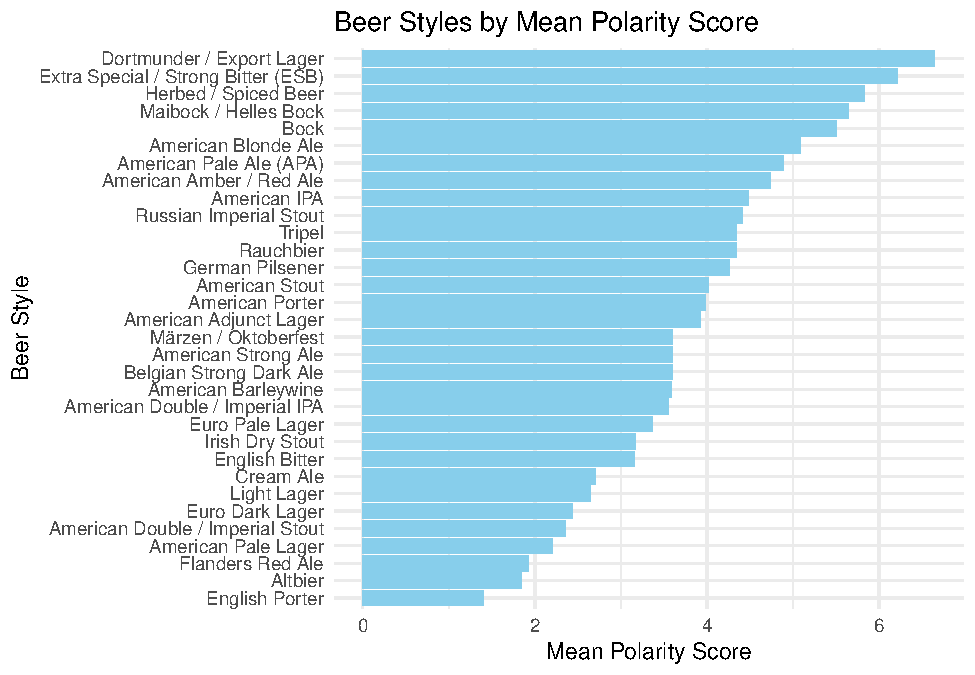
\includegraphics{finalfrfr_files/figure-latex/unnamed-chunk-22-1.pdf}

\begin{Shaded}
\begin{Highlighting}[]
\NormalTok{reviewTextData[reviewTextData}\SpecialCharTok{$}\NormalTok{beer\_style }\SpecialCharTok{==} \StringTok{\textquotesingle{}Dortmunder / Export Lager\textquotesingle{}}\NormalTok{, ]}
\end{Highlighting}
\end{Shaded}

\begin{verbatim}
##     beer_beerId   beer_name beer_ABV                beer_style review_overall
## 727        1415 Amstel Gold        7 Dortmunder / Export Lager              4
##                                                                                                                                                                                                                                                                                                                                                                                                                                   review_text
## 727 Crystal clear sunshine gold, lots of fizzy carbonation adding to a nice white head. Good lacing. Sugary cane and Belgium yeast in the aroma. Some spices and coriander fill the taste profile, a nice sipping 7% brew. I could go for more that one easily, a decent brew, not overpowering at any aspect. Another fresh brew, thanks to my great son, studying overseas in Amsterdam. I was brought this for the unique chance to enjoy.
##                                                                                                                                                                                                                                                                                                                                                                                                                    preprocessed_review_text
## 727 Crystal clear sunshine gold, lots of fizzy carbonation adding to a nice white head. Good lacing. Sugary cane and Belgium yeast in the aroma. Some spices and coriander fill the taste profile, a nice sipping  brew. I could go for more that one easily, a decent brew, not overpowering at any aspect. Another fresh brew, thanks to my great son, studying overseas in Amsterdam. I was brought this for the unique chance to enjoy.
##     polarity_score2
## 727            6.65
\end{verbatim}

\begin{Shaded}
\begin{Highlighting}[]
\NormalTok{reviewTextData[reviewTextData}\SpecialCharTok{$}\NormalTok{beer\_style }\SpecialCharTok{==} \StringTok{\textquotesingle{}Herbed / Spiced Beer\textquotesingle{}}\NormalTok{, ]}
\end{Highlighting}
\end{Shaded}

\begin{verbatim}
##     beer_beerId           beer_name beer_ABV           beer_style
## 1         52159 Caldera Ginger Beer      4.7 Herbed / Spiced Beer
## 58        52159 Caldera Ginger Beer      4.7 Herbed / Spiced Beer
## 324       52159 Caldera Ginger Beer      4.7 Herbed / Spiced Beer
## 325       52159 Caldera Ginger Beer      4.7 Herbed / Spiced Beer
## 326       52159 Caldera Ginger Beer      4.7 Herbed / Spiced Beer
##     review_overall
## 1              5.0
## 58             4.5
## 324            4.0
## 325            4.0
## 326            4.0
##                                                                                                                                                                                                                                                                                                                                                                                                                                                                                                                                                                                                                                                                                                                                                                                                                                                                                                                                                                                                                                                                                                                                                                                                                                                                                                                                                                                                                                                                                                                                                                                                                                                                                                                                                                                                                                                                                                                                                                                                                                                                                                                                               review_text
## 1   OK, so the only reason I bought this while shopping at Whole Foods was because I've never had a "ginger beer" unless it was ginger ALE...and we all know that's not the kind of "beer" we're interested in on this site! I was very excited to try this one!... When poured out it looks like a cheapo macro lager at first sight, then the slowly fading head suggests otherwise. The body is crystal clear and is a very light straw color. The head is bright white and slowly dissipates, but is initially quite thick. Smell is adjuncty, but there are slight notes of honey and some kind of herby thing going on...ginger perhaps? Can't really tell. From the smell there is obviously something different about this beer though. It has a unique spicy smell to it and reminds me a lot of basil, not ginger. I really can't quite place everything that I smell, but it is a very nice aroma. Superb fragrance for this beer, though definitely not a "ginger beer" based on the smell. The taste is very unique also. It's kind of like a spiced pilsner or kolsch but the "spice" is kind of hard to identify. It does not taste like ginger. This beer actually reminds me a lot of Bison's Honey Basil ale. There is some definite astringent burn in the upper throat after swallowing that is no doubt from the ginger, but that is the only ginger I can detect with any certainty. It is only slightly hoppy and malty. This a very enjoyable, very drinkable beer (I could easily drink 2 22oz'ers) but I think it's failing in its claim to be a "ginger" beer because I don't smell it, can barely taste it, and can only really detect the ginger's physiological effects of a warm throat and stomach. So, rating this one is hard; I've never had a ginger beer so I don't really know what one ought to taste like...but then again I can't really tell if I'm tasting ginger here or the combination of other things. So confused. My recommendation to you Caldera folks: ADD MORE GINGER! There's obviously enough of a curiosity about this style to not hurt sales if it was strengthened. I for one could handle it.
## 58                                                                                                                                                                                                                                                                                                                                                                                                                                                                                                                                                                                                                                                                                                                                                                                                                                                                                                                                                                                                                                                                                  Poured from a 22oz bomber into my Drie Fonteinen tumbler. Hazy titanium yellow body (which catches the shadows forming a beautiful mysterious gradient) with an incredibly dense pillow of magnolia cream. Heavy persistent head and rich creamy lacing. Pale malt, asian pear, and a hint of citrus in the nose. A vaguely tropical lager... Tastes very much like a well done APA, with a nice balance of pale malt and low hop bitterness. The ginger adds to the refreshing character, but isn't readily detectable at first (lacks any "bite"). Medium-dry finish - very clean and extremely quaffable. I can imagine hibiscus and beets working in small quantities, though I think they omitted those for this version... Light bodied, pillowy, smooth and moderately carbonated. Don't go into this expecting a ginger beer (despite its name) as it has little in common with that spicy soft drink. This is a wonderful session ale though, and worth seeking out if you are a fan of light yet flavorful lagers. Would obviously go perfectly with sushi.
## 324                                                                                                                                                                                                                                                                                                                                                                                                                                                                                                                                                                                                                                                                                                                                                                                                                                                                                                                                                                                                                                                                                                                                                                                                                                                                                                                                                                                                                                                                                                                                                                                                                                                              I'm not sure why I picked this up... I like ginger, and it was reasonably cheap compared to the other beers I was looking at. Pours a pale golden color with smallish head. Nose is largely uneventful, some ginger in there, a bit of pear, but mainly normal lager. Taste is pretty good, bringing a bit more of the ginger to the fore. MF was a bit fizzy, not terrible though. Easy drinker, I had no problem finishing the bomber. Interesting, but I probably won't get it again.
## 325                                                                                                                                                                                                                                                                                                                                                                                                                                                                                                                                                                                                                                                                                                                                                                                                                                                                                                                                                                                                                                                                                                                                                                                                                                                                                                                                                                                                                                                                                            Notes from 6/24 A: Bright golden glowing beer in a moment of clarity with a lively white head of feathery fluff S: The ginger is definitely there, or am I smelling my Indian dinner? Almost cake-like in its malt aroma, sharply bready with a slight edge of sweetness T: Nice clear malty throat taste, reminds me of strands of complex sugars and grains, ginger is more subtle than I expected, more of an undertone than a backbone M: A refreshing light beer feel, like a pilsner or summer ale D: If this was a sixer instead of a double-deuce, I could see this being a fine picnic pounder Overall, pretty impressed for the particular style
## 326                                                                                                                                                                                                                                                                                                                                                                                                                                                                                                                                                                                                                                                                                                                                                                                                                                                                                                                                                                                                                                                                                                                                                                                                                                                                                                                                                                                                                                                                                                                                                                                   22 oz. bomber, A: Pours a clear yellow with a mild white head, good retention. S: Great nose of ginger, honey, perfume. T: Rather light upfront, it reminds me of Lawnmower, with a hint of ale fruitiness/Kolsch-like almost. Good ginger honey notes on the back end, not taking over the beer in any way. The ginger flavour is clear, but I wanted it to come out a little more in the end. M: Very light-bodied, watery, light base beer for sure. D: An easy drinking spiced beer, this will offend no one, but there's not a complexity to this brew at all.
##                                                                                                                                                                                                                                                                                                                                                                                                                                                                                                                                                                                                                                                                                                                                                                                                                                                                                                                                                                                                                                                                                                                                                                                                                                                                                                                                                                                                                                                                                                                                                                                                                                                                                                                                                                                                                                                                                                                                                                                                                                                                                                                                           preprocessed_review_text
## 1   OK, so the only reason I bought this while shopping at Whole Foods was because I have never had a "ginger beer" unless it was ginger ALE...and we all know that is not the kind of "beer" we are interested in on this site! I was very excited to try this one!... When poured out it looks like a cheapo macro lager at first sight, then the slowly fading head suggests otherwise. The body is crystal clear and is a very light straw color. The head is bright white and slowly dissipates, but is initially quite thick. Smell is adjuncty, but there are slight notes of honey and some kind of herby thing going on...ginger perhaps? Ca not really tell. From the smell there is obviously something different about this beer though. It has a unique spicy smell to it and reminds me a lot of basil, not ginger. I really can not quite place everything that I smell, but it is a very nice aroma. Superb fragrance for this beer, though definitely not a "ginger beer" based on the smell. The taste is very unique also. It is kind of like a spiced pilsner or kolsch but the "spice" is kind of hard to identify. It does not taste like ginger. This beer actually reminds me a lot of Bison is Honey Basil ale. There is some definite astringent burn in the upper throat after swallowing that is no doubt from the ginger, but that is the only ginger I can detect with any certainty. It is only slightly hoppy and malty. This a very enjoyable, very drinkable beer (I could easily drink   but I think it is failing in its claim to be a "ginger" beer because I do not smell it, can barely taste it, and can only really detect the ginger is physiological effects of a warm throat and stomach. So, rating this one is hard; I have never had a ginger beer so I do not really know what one ought to taste like...but then again I can not really tell if I am tasting ginger here or the combination of other things. So confused. My recommendation to you Caldera folks: ADD MORE GINGER! There is obviously enough of a curiosity about this style to not hurt sales if it was strengthened. I for one could handle it.
## 58                                                                                                                                                                                                                                                                                                                                                                                                                                                                                                                                                                                                                                                                                                                                                                                                                                                                                                                                                                                                                                                                                             Poured from a  bomber into my Drie Fonteinen tumbler. Hazy titanium yellow body (which catches the shadows forming a beautiful mysterious gradient) with an incredibly dense pillow of magnolia cream. Heavy persistent head and rich creamy lacing. Pale malt, asian pear, and a hint of citrus in the nose. A vaguely tropical lager... Tastes very much like a well done APA, with a nice balance of pale malt and low hop bitterness. The ginger adds to the refreshing character, but is not readily detectable at first (lacks any "bite"). Medium-dry finish - very clean and extremely quaffable. I can imagine hibiscus and beets working in small quantities, though I think they omitted those for this version... Light bodied, pillowy, smooth and moderately carbonated. Do not go into this expecting a ginger beer (despite its name) as it has little in common with that spicy soft drink. This is a wonderful session ale though, and worth seeking out if you are a fan of light yet flavorful lagers. Would obviously go perfectly with sushi.
## 324                                                                                                                                                                                                                                                                                                                                                                                                                                                                                                                                                                                                                                                                                                                                                                                                                                                                                                                                                                                                                                                                                                                                                                                                                                                                                                                                                                                                                                                                                                                                                                                                                                                                   I am not sure why I picked this up... I like ginger, and it was reasonably cheap compared to the other beers I was looking at. Pours a pale golden color with smallish head. Nose is largely uneventful, some ginger in there, a bit of pear, but mainly normal lager. Taste is pretty good, bringing a bit more of the ginger to the fore. MF was a bit fizzy, not terrible though. Easy drinker, I had no problem finishing the bomber. Interesting, but I probably will not get it again.
## 325                                                                                                                                                                                                                                                                                                                                                                                                                                                                                                                                                                                                                                                                                                                                                                                                                                                                                                                                                                                                                                                                                                                                                                                                                                                                                                                                                                                                                                                                                                         Notes from  A: Bright golden glowing beer in a moment of clarity with a lively white head of feathery fluff S: The ginger is definitely there, or am I smelling my Indian dinner? Almost cake-like in its malt aroma, sharply bready with a slight edge of sweetness T: Nice clear malty throat taste, reminds me of strands of complex sugars and grains, ginger is more subtle than I expected, more of an undertone than a backbone M: A refreshing light beer feel, like a pilsner or summer ale D: If this was a sixer instead of a double-deuce, I could see this being a fine picnic pounder Overall, pretty impressed for the particular style
## 326                                                                                                                                                                                                                                                                                                                                                                                                                                                                                                                                                                                                                                                                                                                                                                                                                                                                                                                                                                                                                                                                                                                                                                                                                                                                                                                                                                                                                                                                                                                                                                                              oz. bomber, A: Pours a clear yellow with a mild white head, good retention. S: Great nose of ginger, honey, perfume. T: Rather light upfront, it reminds me of Lawnmower, with a hint of ale fruitiness/Kolsch-like almost. Good ginger honey notes on the back end, not taking over the beer in any way. The ginger flavour is clear, but I wanted it to come out a little more in the end. M: Very light-bodied, watery, light base beer for sure. D: An easy drinking spiced beer, this will offend no one, but there is not a complexity to this brew at all.
##     polarity_score2
## 1              8.10
## 58             7.45
## 324            2.20
## 325            8.20
## 326            3.20
\end{verbatim}

\begin{Shaded}
\begin{Highlighting}[]
\NormalTok{reviewTextData[reviewTextData}\SpecialCharTok{$}\NormalTok{beer\_style }\SpecialCharTok{==} \StringTok{\textquotesingle{}Extra Special / Strong Bitter (ESB)\textquotesingle{}}\NormalTok{, ]}
\end{Highlighting}
\end{Shaded}

\begin{verbatim}
##     beer_beerId beer_name beer_ABV                          beer_style
## 52         6824    E.S.B.      5.6 Extra Special / Strong Bitter (ESB)
## 53         6824    E.S.B.      5.6 Extra Special / Strong Bitter (ESB)
## 306        6824    E.S.B.      5.6 Extra Special / Strong Bitter (ESB)
## 786        6824    E.S.B.      5.6 Extra Special / Strong Bitter (ESB)
## 787        6824    E.S.B.      5.6 Extra Special / Strong Bitter (ESB)
## 788        6824    E.S.B.      5.6 Extra Special / Strong Bitter (ESB)
##     review_overall
## 52             5.0
## 53             5.0
## 306            4.5
## 786            4.0
## 787            4.0
## 788            4.0
##                                                                                                                                                                                                                                                                                                                                                                                                                                                                                                                                                                                                                                                                                                                                                                                                                                                                                                                                                                                                                                                                                                                                                                                                                                                                                                                                                                                                                                                                                                                                                                                                                                                                                                                                                                    review_text
## 52                                                                                                                                                                                                                                                                                                                                                                                                                                                                                                                                                                                                                                                                                                                                                                                                                                                                                                                        A - It pours in an exceptionally picturesque manner. Never have I seen a cask beer look so good. The brown body proudly boasts a generous crown of off-white frothy head. I am astounded. S - Amazing, fantastic, beyond superlative. Delectable notes of cocoa and vanilla mingle with a rich maltiness and a bright grassy-leafy hop bitterness. T - This beer is loaded with complexity and subtlety; it is also the picture of balance. The earthy, leafy, grassy and resiny hop is very forward in the mix, but the malt is ample and sturdy. Notes of rich malt meld into nuances of vanilla and cocoa, and the hop segues from bitter to more herbal as the glass empties. M - Velvety and luxurious, with ample brightness and effervescence. The best cask I've ever had. D - I would drink many a pint of this if I lived in Indianapolis.
## 53  When I was new to microbrews, I went to any microbrew and tried the sampler, and usually ended up with the dark beers. I had never had an ESB at this point, and didn't really know what the hell it was. Well, the Cumberland in Louisville brewed one and I tried it, and shrugged. It was lighter, but I preferred thier pale and nitro porter. So my friend and I were in the Broad Ripple, and I had thier dark beer, but he had the ESB because he was more experienced with beers. He said I should get one, so I did. That was it. I locked into it and drank nothing else when I went to the Broad Ripple. Period. It was the best ESB that I compared all others too. This past weekend, five years with two years of being a BA later, I found myself at the Broad Ripple and ordered the holy grail of ESB's and well, it wasn't as wonderful as I remembered, but then, as I sipped, it became again, a great beer in my book. It had a good head that stayed with the beer and was a cloudy yellow-grey appearence, almost like a mead. There was not much to smell, but the grains used. Not as pungent as a wheat or Hefe. Mouth was watery, not much bite, washed down clean with good foam , it was also served near room temperature. Taste was, well, very decent. It wasn't as hoppy as some American ESBs, it had a mild flavor with a slight bitter wash, but what made this beer was the flavor of the grains used. I could almost pick out the elements in this beer, and imagined that if I ordered an ESB in a bar in England, this is the pint I'd get. Very nice. Well, ESB from Broad Ripple remains the finest microbrewed ESB with only Fullers ESB in bottles being the best I've tried. If you're at the BR, get one. Then, get another.
## 306                                                                                                                                                                                                                                                                                                                                                                                                                                                                                                                                                                                                                                                                                                                                                                                                                                                                                                                                                                                                                                                                                                                                                                                                                                                                                                                                                                                                                                                                      Nice ESB, it had a wonderful copper color to it, with excellent lacing. Nice malty scent, and a nice bit of earthy hops in the undertone. Good taste, nice and clean, with a bit more of a malty feel than most ESBs, with a wonderful earthy hop finish. It goes down smooth, quite a wonderful ESB.
## 786                                                                                                                                                                                                                                                                                                                                                                                                                                                                                                                                                                                                                                                                                                                                                                                                                                                                                                                                                                                                                                                                                                                                                                                                                                                                                                                                                                                                                 This was the best beer I had at Broad Ripple when I was recently there. This is a great example of a Bitter: hazy golden color, moderate lacing, great smell (biting hops) and the taste is amazing. Perfectly balanced malt and hops; not too bitter and just the right amount of fruity sweetness. This and their double IPA go great with fish'n'chips.
## 787                                                                                                                                                                                                                                                                                                                                                                                                                                                                                                                                                                                                                                                                                                                                                                                                                                                                                                                                                                                                                                                                                                                                                                                                                                                                                                                                                                       Copper colored and slightly hazy. Not much head to speak of. Aroma is malty sweetness. Big hop flavor and aftertaste, but it does not overpower the malt backbone. Hop flavor is a bit woody. Medium bodied. The menu says this beer won a gold at the GABF. It is a good beer, but I have to say of all those I sampled I liked the Replic Ale (Cask-conditioned Scottish-80) better than the rest.
## 788                                                                                                                                                                                                                                                                                                                                                                                                                                                                                                                                                                                                                                                                                                                                                                                                                                                                                                                                                                                         (Served in a pint glass) A- This beer has a warm reddish-brown body with a thick snow-white head that last for a bit then fades to a thin ring around the rim. There is a gentle carbonation of tiny bubbles. S- The taste of smooth toasted malt has a very slight sweetness to it giving it a fresh taste with a light pine hops nose to follow. T- The flavor of toasted malt is supported by notes of biscuit malt and a very light caramel note. The finish is a light smooth pine hops with a light bitterness that finishes pretty quickly. M- This beer has a medium mouthfeel with a soft alcohol warmth when the beer warms. D- This beer has some nice malt flavor with softer hop flavor. This is a nice session beer with good malt flavors supported by hops flavor.
##                                                                                                                                                                                                                                                                                                                                                                                                                                                                                                                                                                                                                                                                                                                                                                                                                                                                                                                                                                                                                                                                                                                                                                                                                                                                                                                                                                                                                                                                                                                                                                                                                                                                                                                                                                  preprocessed_review_text
## 52                                                                                                                                                                                                                                                                                                                                                                                                                                                                                                                                                                                                                                                                                                                                                                                                                                                                                                                                 A - It pours in an exceptionally picturesque manner. Never have I seen a cask beer look so good. The brown body proudly boasts a generous crown of off-white frothy head. I am astounded. S - Amazing, fantastic, beyond superlative. Delectable notes of cocoa and vanilla mingle with a rich maltiness and a bright grassy-leafy hop bitterness. T - This beer is loaded with complexity and subtlety; it is also the picture of balance. The earthy, leafy, grassy and resiny hop is very forward in the mix, but the malt is ample and sturdy. Notes of rich malt meld into nuances of vanilla and cocoa, and the hop segues from bitter to more herbal as the glass empties. M - Velvety and luxurious, with ample brightness and effervescence. The best cask I have ever had. D - I would drink many a pint of this if I lived in Indianapolis.
## 53  When I was new to microbrews, I went to any microbrew and tried the sampler, and usually ended up with the dark beers. I had never had an ESB at this point, and did not really know what the hell it was. Well, the Cumberland in Louisville brewed one and I tried it, and shrugged. It was lighter, but I preferred thier pale and nitro porter. So my friend and I were in the Broad Ripple, and I had thier dark beer, but he had the ESB because he was more experienced with beers. He said I should get one, so I did. That was it. I locked into it and drank nothing else when I went to the Broad Ripple. Period. It was the best ESB that I compared all others too. This past weekend, five years with two years of being a BA later, I found myself at the Broad Ripple and ordered the holy grail of ESB is and well, it was not as wonderful as I remembered, but then, as I sipped, it became again, a great beer in my book. It had a good head that stayed with the beer and was a cloudy yellow-grey appearence, almost like a mead. There was not much to smell, but the grains used. Not as pungent as a wheat or Hefe. Mouth was watery, not much bite, washed down clean with good foam , it was also served near room temperature. Taste was, well, very decent. It was not as hoppy as some American ESBs, it had a mild flavor with a slight bitter wash, but what made this beer was the flavor of the grains used. I could almost pick out the elements in this beer, and imagined that if I ordered an ESB in a bar in England, this is the pint I would get. Very nice. Well, ESB from Broad Ripple remains the finest microbrewed ESB with only Fullers ESB in bottles being the best I have tried. If you are at the BR, get one. Then, get another.
## 306                                                                                                                                                                                                                                                                                                                                                                                                                                                                                                                                                                                                                                                                                                                                                                                                                                                                                                                                                                                                                                                                                                                                                                                                                                                                                                                                                                                                                                                                                 Nice ESB, it had a wonderful copper color to it, with excellent lacing. Nice malty scent, and a nice bit of earthy hops in the undertone. Good taste, nice and clean, with a bit more of a malty feel than most ESBs, with a wonderful earthy hop finish. It goes down smooth, quite a wonderful ESB.
## 786                                                                                                                                                                                                                                                                                                                                                                                                                                                                                                                                                                                                                                                                                                                                                                                                                                                                                                                                                                                                                                                                                                                                                                                                                                                                                                                                                                                                                            This was the best beer I had at Broad Ripple when I was recently there. This is a great example of a Bitter: hazy golden color, moderate lacing, great smell (biting hops) and the taste is amazing. Perfectly balanced malt and hops; not too bitter and just the right amount of fruity sweetness. This and their double IPA go great with fish'n'chips.
## 787                                                                                                                                                                                                                                                                                                                                                                                                                                                                                                                                                                                                                                                                                                                                                                                                                                                                                                                                                                                                                                                                                                                                                                                                                                                                                                                                                                                              Copper colored and slightly hazy. Not much head to speak of. Aroma is malty sweetness. Big hop flavor and aftertaste, but it does not overpower the malt backbone. Hop flavor is a bit woody. Medium bodied. The menu says this beer won a gold at the GABF. It is a good beer, but I have to say of all those I sampled I liked the Replic Ale (Cask-conditioned  better than the rest.
## 788                                                                                                                                                                                                                                                                                                                                                                                                                                                                                                                                                                                                                                                                                                                                                                                                                                                                                                                                                                                                    (Served in a pint glass) A- This beer has a warm reddish-brown body with a thick snow-white head that last for a bit then fades to a thin ring around the rim. There is a gentle carbonation of tiny bubbles. S- The taste of smooth toasted malt has a very slight sweetness to it giving it a fresh taste with a light pine hops nose to follow. T- The flavor of toasted malt is supported by notes of biscuit malt and a very light caramel note. The finish is a light smooth pine hops with a light bitterness that finishes pretty quickly. M- This beer has a medium mouthfeel with a soft alcohol warmth when the beer warms. D- This beer has some nice malt flavor with softer hop flavor. This is a nice session beer with good malt flavors supported by hops flavor.
##     polarity_score2
## 52            11.95
## 53             6.45
## 306            4.35
## 786            3.90
## 787            2.75
## 788            7.90
\end{verbatim}

\begin{Shaded}
\begin{Highlighting}[]
\CommentTok{\# q5 ans. by observing the mean compound polarity score , the beer style "Dortmunder / Export Lager" is liked most but has only one review that likes it as much, instead we can say "Extra Special / Strong Bitter (ESB)" is the most famous, based on combination of polarity and higher frequency}
\end{Highlighting}
\end{Shaded}

\begin{Shaded}
\begin{Highlighting}[]
\CommentTok{\# create a scatter plot comparing polarity score with overall review score}
\FunctionTok{ggplot}\NormalTok{(}\AttributeTok{data =}\NormalTok{ reviewTextData, }\FunctionTok{aes}\NormalTok{(}\AttributeTok{x =}\NormalTok{ polarity\_score2, }\AttributeTok{y =}\NormalTok{ review\_overall)) }\SpecialCharTok{+}
  \FunctionTok{geom\_point}\NormalTok{(}\AttributeTok{color =} \StringTok{"blue"}\NormalTok{, }\AttributeTok{alpha =} \FloatTok{0.6}\NormalTok{) }\SpecialCharTok{+}
  \FunctionTok{labs}\NormalTok{(}\AttributeTok{title =} \StringTok{"Relationship between Polarity Score and Overall Review Score"}\NormalTok{,}
       \AttributeTok{x =} \StringTok{"Polarity Score"}\NormalTok{,}
       \AttributeTok{y =} \StringTok{"Overall Review Score"}\NormalTok{) }\SpecialCharTok{+}
  \FunctionTok{theme\_minimal}\NormalTok{()}
\end{Highlighting}
\end{Shaded}

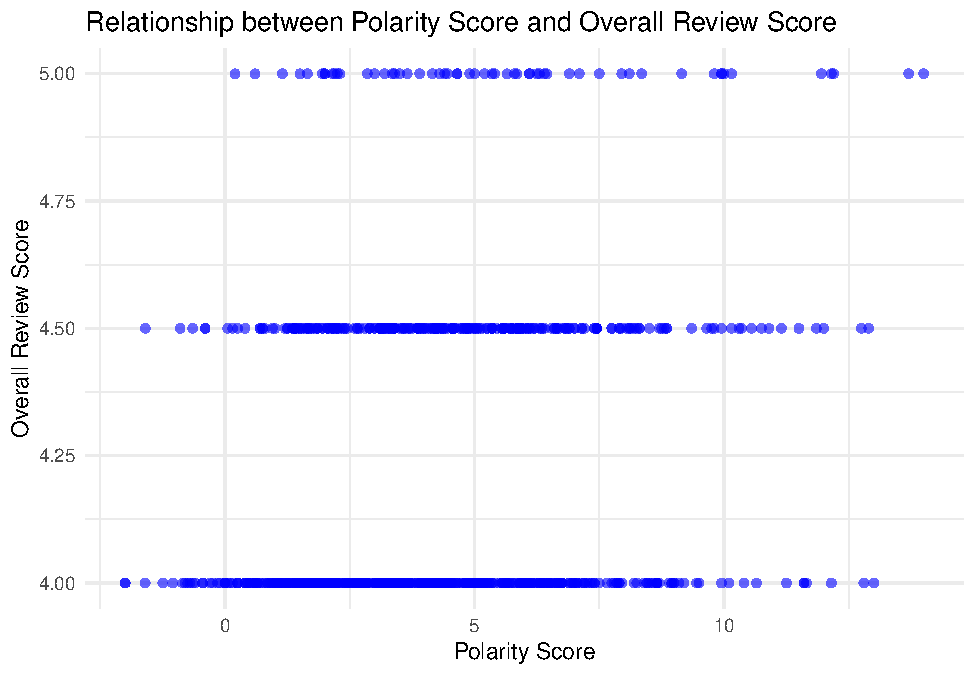
\includegraphics{finalfrfr_files/figure-latex/unnamed-chunk-25-1.pdf}

\begin{Shaded}
\begin{Highlighting}[]
\CommentTok{\# q6 ans. by observing the mean compound polarity score calculated we can get an idea how the user written review text is collaborating in calculating the overall review score, as seen in graph there is little to no correlation so the text reviews or overall review scores are unreliable on their own}
\end{Highlighting}
\end{Shaded}

\begin{Shaded}
\begin{Highlighting}[]
\CommentTok{\# 7. How to find similar beer drinkers by using written reviews only?}
\CommentTok{\# using ML techniques}
\FunctionTok{library}\NormalTok{(tm)}
\end{Highlighting}
\end{Shaded}

\begin{verbatim}
## Loading required package: NLP
\end{verbatim}

\begin{verbatim}
## 
## Attaching package: 'NLP'
\end{verbatim}

\begin{verbatim}
## The following object is masked from 'package:ggplot2':
## 
##     annotate
\end{verbatim}

\begin{Shaded}
\begin{Highlighting}[]
\FunctionTok{library}\NormalTok{(proxy)}
\end{Highlighting}
\end{Shaded}

\begin{verbatim}
## 
## Attaching package: 'proxy'
\end{verbatim}

\begin{verbatim}
## The following objects are masked from 'package:stats':
## 
##     as.dist, dist
\end{verbatim}

\begin{verbatim}
## The following object is masked from 'package:base':
## 
##     as.matrix
\end{verbatim}

\begin{Shaded}
\begin{Highlighting}[]
\CommentTok{\# Create a term{-}document matrix using TF{-}IDF}
\NormalTok{tdm }\OtherTok{\textless{}{-}} \FunctionTok{DocumentTermMatrix}\NormalTok{(}\FunctionTok{Corpus}\NormalTok{(}\FunctionTok{VectorSource}\NormalTok{(reviewTextData}\SpecialCharTok{$}\NormalTok{preprocessed\_review\_text)),}
                          \AttributeTok{control =} \FunctionTok{list}\NormalTok{(}\AttributeTok{weighting =} \ControlFlowTok{function}\NormalTok{(x) }\FunctionTok{weightTfIdf}\NormalTok{(x, }\AttributeTok{normalize =} \ConstantTok{TRUE}\NormalTok{)))}
\end{Highlighting}
\end{Shaded}

\begin{verbatim}
## Warning in TermDocumentMatrix.SimpleCorpus(x, control): custom functions are
## ignored
\end{verbatim}

\begin{Shaded}
\begin{Highlighting}[]
\CommentTok{\# Convert the term{-}document matrix to a matrix}
\NormalTok{tfidf\_matrix }\OtherTok{\textless{}{-}} \FunctionTok{as.matrix}\NormalTok{(tdm)}

\CommentTok{\# Calculate cosine similarity between user reviews}
\NormalTok{cosine\_similarities }\OtherTok{\textless{}{-}}\NormalTok{ proxy}\SpecialCharTok{::}\FunctionTok{simil}\NormalTok{(tfidf\_matrix, tfidf\_matrix, }\AttributeTok{method =} \StringTok{"cosine"}\NormalTok{, }\AttributeTok{upper =} \ConstantTok{TRUE}\NormalTok{)}
\end{Highlighting}
\end{Shaded}

\begin{Shaded}
\begin{Highlighting}[]
\CommentTok{\# load necessary library}
\FunctionTok{library}\NormalTok{(stats)}

\CommentTok{\# grouping together similar customers based on reviews}
\NormalTok{kmeans\_model }\OtherTok{\textless{}{-}} \FunctionTok{kmeans}\NormalTok{(cosine\_similarities, }\AttributeTok{centers =} \DecValTok{4}\NormalTok{)}
\NormalTok{clusters }\OtherTok{\textless{}{-}}\NormalTok{ kmeans\_model}\SpecialCharTok{$}\NormalTok{cluster}

\CommentTok{\# analyze cluster assignments}
\CommentTok{\# assign each user to a cluster}
\NormalTok{user\_clusters }\OtherTok{\textless{}{-}} \FunctionTok{list}\NormalTok{()}

\ControlFlowTok{for}\NormalTok{ (user\_id }\ControlFlowTok{in} \DecValTok{1}\SpecialCharTok{:}\FunctionTok{length}\NormalTok{(clusters)) \{}
\NormalTok{  cluster\_id }\OtherTok{\textless{}{-}}\NormalTok{ clusters[user\_id]}
  \ControlFlowTok{if}\NormalTok{ (}\SpecialCharTok{!}\NormalTok{(}\FunctionTok{as.character}\NormalTok{(cluster\_id) }\SpecialCharTok{\%in\%} \FunctionTok{names}\NormalTok{(user\_clusters))) \{}
\NormalTok{    user\_clusters[[}\FunctionTok{as.character}\NormalTok{(cluster\_id)]] }\OtherTok{\textless{}{-}} \FunctionTok{c}\NormalTok{()}
\NormalTok{  \}}
\NormalTok{  user\_clusters[[}\FunctionTok{as.character}\NormalTok{(cluster\_id)]] }\OtherTok{\textless{}{-}} \FunctionTok{c}\NormalTok{(user\_clusters[[}\FunctionTok{as.character}\NormalTok{(cluster\_id)]], user\_id)}
\NormalTok{\}}

\CommentTok{\# print the users in each cluster}
\ControlFlowTok{for}\NormalTok{ (cluster\_id }\ControlFlowTok{in} \FunctionTok{names}\NormalTok{(user\_clusters)) \{}
  \FunctionTok{cat}\NormalTok{(}\FunctionTok{paste}\NormalTok{(}\StringTok{"Cluster"}\NormalTok{, cluster\_id, }\StringTok{":"}\NormalTok{, user\_clusters[[cluster\_id]], }\StringTok{"}\SpecialCharTok{\textbackslash{}n}\StringTok{"}\NormalTok{))}
\NormalTok{\}}
\end{Highlighting}
\end{Shaded}

\begin{verbatim}
## Cluster 4 : 1 
##  Cluster 4 : 5 
##  Cluster 4 : 7 
##  Cluster 4 : 9 
##  Cluster 4 : 10 
##  Cluster 4 : 12 
##  Cluster 4 : 13 
##  Cluster 4 : 19 
##  Cluster 4 : 22 
##  Cluster 4 : 28 
##  Cluster 4 : 31 
##  Cluster 4 : 32 
##  Cluster 4 : 35 
##  Cluster 4 : 36 
##  Cluster 4 : 43 
##  Cluster 4 : 44 
##  Cluster 4 : 53 
##  Cluster 4 : 61 
##  Cluster 4 : 65 
##  Cluster 4 : 66 
##  Cluster 4 : 67 
##  Cluster 4 : 69 
##  Cluster 4 : 70 
##  Cluster 4 : 86 
##  Cluster 4 : 92 
##  Cluster 4 : 93 
##  Cluster 4 : 101 
##  Cluster 4 : 102 
##  Cluster 4 : 105 
##  Cluster 4 : 109 
##  Cluster 4 : 111 
##  Cluster 4 : 117 
##  Cluster 4 : 121 
##  Cluster 4 : 126 
##  Cluster 4 : 131 
##  Cluster 4 : 132 
##  Cluster 4 : 144 
##  Cluster 4 : 146 
##  Cluster 4 : 149 
##  Cluster 4 : 150 
##  Cluster 4 : 152 
##  Cluster 4 : 168 
##  Cluster 4 : 178 
##  Cluster 4 : 180 
##  Cluster 4 : 187 
##  Cluster 4 : 190 
##  Cluster 4 : 191 
##  Cluster 4 : 217 
##  Cluster 4 : 221 
##  Cluster 4 : 230 
##  Cluster 4 : 232 
##  Cluster 4 : 239 
##  Cluster 4 : 246 
##  Cluster 4 : 249 
##  Cluster 4 : 252 
##  Cluster 4 : 254 
##  Cluster 4 : 265 
##  Cluster 4 : 272 
##  Cluster 4 : 275 
##  Cluster 4 : 277 
##  Cluster 4 : 284 
##  Cluster 4 : 293 
##  Cluster 4 : 294 
##  Cluster 4 : 295 
##  Cluster 4 : 297 
##  Cluster 4 : 301 
##  Cluster 4 : 323 
##  Cluster 4 : 332 
##  Cluster 4 : 335 
##  Cluster 4 : 343 
##  Cluster 4 : 354 
##  Cluster 4 : 360 
##  Cluster 4 : 363 
##  Cluster 4 : 364 
##  Cluster 4 : 368 
##  Cluster 4 : 369 
##  Cluster 4 : 371 
##  Cluster 4 : 374 
##  Cluster 4 : 381 
##  Cluster 4 : 388 
##  Cluster 4 : 390 
##  Cluster 4 : 398 
##  Cluster 4 : 401 
##  Cluster 4 : 420 
##  Cluster 4 : 426 
##  Cluster 4 : 432 
##  Cluster 4 : 447 
##  Cluster 4 : 449 
##  Cluster 4 : 454 
##  Cluster 4 : 489 
##  Cluster 4 : 495 
##  Cluster 4 : 501 
##  Cluster 4 : 502 
##  Cluster 4 : 503 
##  Cluster 4 : 508 
##  Cluster 4 : 510 
##  Cluster 4 : 511 
##  Cluster 4 : 516 
##  Cluster 4 : 521 
##  Cluster 4 : 525 
##  Cluster 4 : 526 
##  Cluster 4 : 528 
##  Cluster 4 : 531 
##  Cluster 4 : 534 
##  Cluster 4 : 552 
##  Cluster 4 : 560 
##  Cluster 4 : 573 
##  Cluster 4 : 576 
##  Cluster 4 : 581 
##  Cluster 4 : 582 
##  Cluster 4 : 589 
##  Cluster 4 : 602 
##  Cluster 4 : 611 
##  Cluster 4 : 624 
##  Cluster 4 : 627 
##  Cluster 4 : 635 
##  Cluster 4 : 645 
##  Cluster 4 : 647 
##  Cluster 4 : 671 
##  Cluster 4 : 702 
##  Cluster 4 : 712 
##  Cluster 4 : 721 
##  Cluster 4 : 725 
##  Cluster 4 : 730 
##  Cluster 4 : 735 
##  Cluster 4 : 737 
##  Cluster 4 : 738 
##  Cluster 4 : 740 
##  Cluster 4 : 741 
##  Cluster 4 : 743 
##  Cluster 4 : 746 
##  Cluster 4 : 749 
##  Cluster 4 : 750 
##  Cluster 4 : 755 
##  Cluster 4 : 758 
##  Cluster 4 : 759 
##  Cluster 4 : 760 
##  Cluster 4 : 761 
##  Cluster 4 : 762 
##  Cluster 4 : 764 
##  Cluster 4 : 768 
##  Cluster 4 : 770 
##  Cluster 4 : 774 
##  Cluster 4 : 775 
##  Cluster 4 : 785 
##  Cluster 4 : 795 
##  Cluster 4 : 802 
## Cluster 2 : 2 
##  Cluster 2 : 3 
##  Cluster 2 : 14 
##  Cluster 2 : 15 
##  Cluster 2 : 16 
##  Cluster 2 : 17 
##  Cluster 2 : 18 
##  Cluster 2 : 27 
##  Cluster 2 : 30 
##  Cluster 2 : 37 
##  Cluster 2 : 38 
##  Cluster 2 : 39 
##  Cluster 2 : 40 
##  Cluster 2 : 41 
##  Cluster 2 : 42 
##  Cluster 2 : 45 
##  Cluster 2 : 46 
##  Cluster 2 : 47 
##  Cluster 2 : 48 
##  Cluster 2 : 49 
##  Cluster 2 : 50 
##  Cluster 2 : 52 
##  Cluster 2 : 55 
##  Cluster 2 : 56 
##  Cluster 2 : 57 
##  Cluster 2 : 59 
##  Cluster 2 : 60 
##  Cluster 2 : 64 
##  Cluster 2 : 68 
##  Cluster 2 : 71 
##  Cluster 2 : 73 
##  Cluster 2 : 74 
##  Cluster 2 : 87 
##  Cluster 2 : 99 
##  Cluster 2 : 112 
##  Cluster 2 : 113 
##  Cluster 2 : 115 
##  Cluster 2 : 116 
##  Cluster 2 : 118 
##  Cluster 2 : 119 
##  Cluster 2 : 120 
##  Cluster 2 : 122 
##  Cluster 2 : 123 
##  Cluster 2 : 124 
##  Cluster 2 : 125 
##  Cluster 2 : 127 
##  Cluster 2 : 128 
##  Cluster 2 : 130 
##  Cluster 2 : 134 
##  Cluster 2 : 135 
##  Cluster 2 : 153 
##  Cluster 2 : 170 
##  Cluster 2 : 176 
##  Cluster 2 : 208 
##  Cluster 2 : 215 
##  Cluster 2 : 223 
##  Cluster 2 : 236 
##  Cluster 2 : 237 
##  Cluster 2 : 240 
##  Cluster 2 : 241 
##  Cluster 2 : 242 
##  Cluster 2 : 245 
##  Cluster 2 : 251 
##  Cluster 2 : 259 
##  Cluster 2 : 261 
##  Cluster 2 : 270 
##  Cluster 2 : 271 
##  Cluster 2 : 273 
##  Cluster 2 : 274 
##  Cluster 2 : 276 
##  Cluster 2 : 278 
##  Cluster 2 : 280 
##  Cluster 2 : 281 
##  Cluster 2 : 282 
##  Cluster 2 : 285 
##  Cluster 2 : 286 
##  Cluster 2 : 287 
##  Cluster 2 : 288 
##  Cluster 2 : 289 
##  Cluster 2 : 290 
##  Cluster 2 : 291 
##  Cluster 2 : 292 
##  Cluster 2 : 296 
##  Cluster 2 : 298 
##  Cluster 2 : 299 
##  Cluster 2 : 300 
##  Cluster 2 : 302 
##  Cluster 2 : 304 
##  Cluster 2 : 310 
##  Cluster 2 : 311 
##  Cluster 2 : 312 
##  Cluster 2 : 313 
##  Cluster 2 : 314 
##  Cluster 2 : 315 
##  Cluster 2 : 316 
##  Cluster 2 : 320 
##  Cluster 2 : 321 
##  Cluster 2 : 322 
##  Cluster 2 : 324 
##  Cluster 2 : 325 
##  Cluster 2 : 326 
##  Cluster 2 : 327 
##  Cluster 2 : 328 
##  Cluster 2 : 329 
##  Cluster 2 : 330 
##  Cluster 2 : 331 
##  Cluster 2 : 333 
##  Cluster 2 : 334 
##  Cluster 2 : 336 
##  Cluster 2 : 337 
##  Cluster 2 : 338 
##  Cluster 2 : 339 
##  Cluster 2 : 340 
##  Cluster 2 : 341 
##  Cluster 2 : 342 
##  Cluster 2 : 344 
##  Cluster 2 : 345 
##  Cluster 2 : 349 
##  Cluster 2 : 350 
##  Cluster 2 : 372 
##  Cluster 2 : 376 
##  Cluster 2 : 385 
##  Cluster 2 : 389 
##  Cluster 2 : 391 
##  Cluster 2 : 394 
##  Cluster 2 : 409 
##  Cluster 2 : 411 
##  Cluster 2 : 416 
##  Cluster 2 : 417 
##  Cluster 2 : 418 
##  Cluster 2 : 419 
##  Cluster 2 : 422 
##  Cluster 2 : 423 
##  Cluster 2 : 424 
##  Cluster 2 : 425 
##  Cluster 2 : 428 
##  Cluster 2 : 429 
##  Cluster 2 : 431 
##  Cluster 2 : 433 
##  Cluster 2 : 434 
##  Cluster 2 : 435 
##  Cluster 2 : 437 
##  Cluster 2 : 438 
##  Cluster 2 : 439 
##  Cluster 2 : 440 
##  Cluster 2 : 442 
##  Cluster 2 : 443 
##  Cluster 2 : 444 
##  Cluster 2 : 446 
##  Cluster 2 : 448 
##  Cluster 2 : 450 
##  Cluster 2 : 451 
##  Cluster 2 : 452 
##  Cluster 2 : 453 
##  Cluster 2 : 496 
##  Cluster 2 : 514 
##  Cluster 2 : 541 
##  Cluster 2 : 548 
##  Cluster 2 : 554 
##  Cluster 2 : 563 
##  Cluster 2 : 567 
##  Cluster 2 : 590 
##  Cluster 2 : 601 
##  Cluster 2 : 631 
##  Cluster 2 : 633 
##  Cluster 2 : 634 
##  Cluster 2 : 636 
##  Cluster 2 : 648 
##  Cluster 2 : 656 
##  Cluster 2 : 657 
##  Cluster 2 : 658 
##  Cluster 2 : 661 
##  Cluster 2 : 670 
##  Cluster 2 : 680 
##  Cluster 2 : 690 
##  Cluster 2 : 694 
##  Cluster 2 : 695 
##  Cluster 2 : 700 
##  Cluster 2 : 705 
##  Cluster 2 : 709 
##  Cluster 2 : 710 
##  Cluster 2 : 711 
##  Cluster 2 : 713 
##  Cluster 2 : 714 
##  Cluster 2 : 715 
##  Cluster 2 : 716 
##  Cluster 2 : 717 
##  Cluster 2 : 718 
##  Cluster 2 : 719 
##  Cluster 2 : 720 
##  Cluster 2 : 722 
##  Cluster 2 : 723 
##  Cluster 2 : 726 
##  Cluster 2 : 727 
##  Cluster 2 : 728 
##  Cluster 2 : 729 
##  Cluster 2 : 731 
##  Cluster 2 : 732 
##  Cluster 2 : 734 
##  Cluster 2 : 736 
##  Cluster 2 : 742 
##  Cluster 2 : 744 
##  Cluster 2 : 745 
##  Cluster 2 : 747 
##  Cluster 2 : 748 
##  Cluster 2 : 751 
##  Cluster 2 : 752 
##  Cluster 2 : 753 
##  Cluster 2 : 754 
##  Cluster 2 : 756 
##  Cluster 2 : 757 
##  Cluster 2 : 763 
##  Cluster 2 : 765 
##  Cluster 2 : 766 
##  Cluster 2 : 767 
##  Cluster 2 : 769 
##  Cluster 2 : 771 
##  Cluster 2 : 772 
##  Cluster 2 : 773 
##  Cluster 2 : 776 
##  Cluster 2 : 778 
##  Cluster 2 : 779 
##  Cluster 2 : 780 
##  Cluster 2 : 781 
##  Cluster 2 : 782 
##  Cluster 2 : 783 
##  Cluster 2 : 786 
##  Cluster 2 : 787 
##  Cluster 2 : 789 
##  Cluster 2 : 790 
##  Cluster 2 : 791 
##  Cluster 2 : 792 
##  Cluster 2 : 793 
##  Cluster 2 : 794 
##  Cluster 2 : 796 
##  Cluster 2 : 797 
##  Cluster 2 : 798 
##  Cluster 2 : 799 
##  Cluster 2 : 800 
##  Cluster 2 : 801 
##  Cluster 2 : 803 
##  Cluster 2 : 804 
##  Cluster 2 : 805 
##  Cluster 2 : 806 
##  Cluster 2 : 807 
##  Cluster 2 : 809 
##  Cluster 2 : 810 
##  Cluster 2 : 811 
##  Cluster 2 : 812 
##  Cluster 2 : 813 
##  Cluster 2 : 814 
##  Cluster 2 : 815 
##  Cluster 2 : 816 
## Cluster 3 : 4 
##  Cluster 3 : 6 
##  Cluster 3 : 8 
##  Cluster 3 : 20 
##  Cluster 3 : 21 
##  Cluster 3 : 23 
##  Cluster 3 : 33 
##  Cluster 3 : 34 
##  Cluster 3 : 51 
##  Cluster 3 : 54 
##  Cluster 3 : 58 
##  Cluster 3 : 62 
##  Cluster 3 : 63 
##  Cluster 3 : 72 
##  Cluster 3 : 75 
##  Cluster 3 : 76 
##  Cluster 3 : 79 
##  Cluster 3 : 80 
##  Cluster 3 : 81 
##  Cluster 3 : 82 
##  Cluster 3 : 85 
##  Cluster 3 : 88 
##  Cluster 3 : 90 
##  Cluster 3 : 94 
##  Cluster 3 : 97 
##  Cluster 3 : 98 
##  Cluster 3 : 103 
##  Cluster 3 : 104 
##  Cluster 3 : 106 
##  Cluster 3 : 108 
##  Cluster 3 : 110 
##  Cluster 3 : 114 
##  Cluster 3 : 129 
##  Cluster 3 : 133 
##  Cluster 3 : 138 
##  Cluster 3 : 141 
##  Cluster 3 : 142 
##  Cluster 3 : 143 
##  Cluster 3 : 145 
##  Cluster 3 : 147 
##  Cluster 3 : 154 
##  Cluster 3 : 155 
##  Cluster 3 : 158 
##  Cluster 3 : 161 
##  Cluster 3 : 162 
##  Cluster 3 : 163 
##  Cluster 3 : 165 
##  Cluster 3 : 167 
##  Cluster 3 : 169 
##  Cluster 3 : 174 
##  Cluster 3 : 175 
##  Cluster 3 : 185 
##  Cluster 3 : 189 
##  Cluster 3 : 192 
##  Cluster 3 : 193 
##  Cluster 3 : 197 
##  Cluster 3 : 199 
##  Cluster 3 : 200 
##  Cluster 3 : 201 
##  Cluster 3 : 202 
##  Cluster 3 : 203 
##  Cluster 3 : 204 
##  Cluster 3 : 205 
##  Cluster 3 : 209 
##  Cluster 3 : 212 
##  Cluster 3 : 214 
##  Cluster 3 : 216 
##  Cluster 3 : 218 
##  Cluster 3 : 222 
##  Cluster 3 : 224 
##  Cluster 3 : 225 
##  Cluster 3 : 226 
##  Cluster 3 : 227 
##  Cluster 3 : 229 
##  Cluster 3 : 233 
##  Cluster 3 : 234 
##  Cluster 3 : 235 
##  Cluster 3 : 248 
##  Cluster 3 : 253 
##  Cluster 3 : 255 
##  Cluster 3 : 256 
##  Cluster 3 : 260 
##  Cluster 3 : 262 
##  Cluster 3 : 263 
##  Cluster 3 : 264 
##  Cluster 3 : 266 
##  Cluster 3 : 268 
##  Cluster 3 : 279 
##  Cluster 3 : 283 
##  Cluster 3 : 303 
##  Cluster 3 : 305 
##  Cluster 3 : 306 
##  Cluster 3 : 307 
##  Cluster 3 : 308 
##  Cluster 3 : 309 
##  Cluster 3 : 317 
##  Cluster 3 : 318 
##  Cluster 3 : 319 
##  Cluster 3 : 346 
##  Cluster 3 : 347 
##  Cluster 3 : 352 
##  Cluster 3 : 357 
##  Cluster 3 : 362 
##  Cluster 3 : 365 
##  Cluster 3 : 366 
##  Cluster 3 : 367 
##  Cluster 3 : 370 
##  Cluster 3 : 375 
##  Cluster 3 : 377 
##  Cluster 3 : 378 
##  Cluster 3 : 379 
##  Cluster 3 : 384 
##  Cluster 3 : 393 
##  Cluster 3 : 395 
##  Cluster 3 : 396 
##  Cluster 3 : 397 
##  Cluster 3 : 400 
##  Cluster 3 : 403 
##  Cluster 3 : 404 
##  Cluster 3 : 405 
##  Cluster 3 : 406 
##  Cluster 3 : 408 
##  Cluster 3 : 410 
##  Cluster 3 : 413 
##  Cluster 3 : 414 
##  Cluster 3 : 415 
##  Cluster 3 : 421 
##  Cluster 3 : 430 
##  Cluster 3 : 436 
##  Cluster 3 : 441 
##  Cluster 3 : 455 
##  Cluster 3 : 457 
##  Cluster 3 : 459 
##  Cluster 3 : 460 
##  Cluster 3 : 461 
##  Cluster 3 : 463 
##  Cluster 3 : 466 
##  Cluster 3 : 467 
##  Cluster 3 : 468 
##  Cluster 3 : 469 
##  Cluster 3 : 471 
##  Cluster 3 : 472 
##  Cluster 3 : 473 
##  Cluster 3 : 476 
##  Cluster 3 : 479 
##  Cluster 3 : 481 
##  Cluster 3 : 483 
##  Cluster 3 : 484 
##  Cluster 3 : 488 
##  Cluster 3 : 491 
##  Cluster 3 : 493 
##  Cluster 3 : 494 
##  Cluster 3 : 500 
##  Cluster 3 : 504 
##  Cluster 3 : 506 
##  Cluster 3 : 507 
##  Cluster 3 : 513 
##  Cluster 3 : 517 
##  Cluster 3 : 518 
##  Cluster 3 : 519 
##  Cluster 3 : 520 
##  Cluster 3 : 527 
##  Cluster 3 : 532 
##  Cluster 3 : 533 
##  Cluster 3 : 535 
##  Cluster 3 : 536 
##  Cluster 3 : 538 
##  Cluster 3 : 539 
##  Cluster 3 : 540 
##  Cluster 3 : 543 
##  Cluster 3 : 544 
##  Cluster 3 : 545 
##  Cluster 3 : 546 
##  Cluster 3 : 550 
##  Cluster 3 : 553 
##  Cluster 3 : 557 
##  Cluster 3 : 558 
##  Cluster 3 : 559 
##  Cluster 3 : 564 
##  Cluster 3 : 565 
##  Cluster 3 : 566 
##  Cluster 3 : 569 
##  Cluster 3 : 570 
##  Cluster 3 : 572 
##  Cluster 3 : 574 
##  Cluster 3 : 578 
##  Cluster 3 : 579 
##  Cluster 3 : 584 
##  Cluster 3 : 585 
##  Cluster 3 : 586 
##  Cluster 3 : 588 
##  Cluster 3 : 591 
##  Cluster 3 : 593 
##  Cluster 3 : 594 
##  Cluster 3 : 596 
##  Cluster 3 : 599 
##  Cluster 3 : 600 
##  Cluster 3 : 603 
##  Cluster 3 : 604 
##  Cluster 3 : 606 
##  Cluster 3 : 607 
##  Cluster 3 : 608 
##  Cluster 3 : 610 
##  Cluster 3 : 612 
##  Cluster 3 : 616 
##  Cluster 3 : 618 
##  Cluster 3 : 620 
##  Cluster 3 : 623 
##  Cluster 3 : 625 
##  Cluster 3 : 629 
##  Cluster 3 : 632 
##  Cluster 3 : 637 
##  Cluster 3 : 639 
##  Cluster 3 : 640 
##  Cluster 3 : 643 
##  Cluster 3 : 644 
##  Cluster 3 : 646 
##  Cluster 3 : 650 
##  Cluster 3 : 652 
##  Cluster 3 : 653 
##  Cluster 3 : 654 
##  Cluster 3 : 655 
##  Cluster 3 : 662 
##  Cluster 3 : 665 
##  Cluster 3 : 668 
##  Cluster 3 : 669 
##  Cluster 3 : 672 
##  Cluster 3 : 673 
##  Cluster 3 : 674 
##  Cluster 3 : 675 
##  Cluster 3 : 676 
##  Cluster 3 : 678 
##  Cluster 3 : 679 
##  Cluster 3 : 681 
##  Cluster 3 : 682 
##  Cluster 3 : 683 
##  Cluster 3 : 686 
##  Cluster 3 : 687 
##  Cluster 3 : 691 
##  Cluster 3 : 692 
##  Cluster 3 : 696 
##  Cluster 3 : 697 
##  Cluster 3 : 698 
##  Cluster 3 : 699 
##  Cluster 3 : 701 
##  Cluster 3 : 703 
##  Cluster 3 : 707 
##  Cluster 3 : 724 
##  Cluster 3 : 733 
##  Cluster 3 : 739 
##  Cluster 3 : 777 
##  Cluster 3 : 784 
##  Cluster 3 : 808 
## Cluster 1 : 11 
##  Cluster 1 : 24 
##  Cluster 1 : 25 
##  Cluster 1 : 26 
##  Cluster 1 : 29 
##  Cluster 1 : 77 
##  Cluster 1 : 78 
##  Cluster 1 : 83 
##  Cluster 1 : 84 
##  Cluster 1 : 89 
##  Cluster 1 : 91 
##  Cluster 1 : 95 
##  Cluster 1 : 96 
##  Cluster 1 : 100 
##  Cluster 1 : 107 
##  Cluster 1 : 136 
##  Cluster 1 : 137 
##  Cluster 1 : 139 
##  Cluster 1 : 140 
##  Cluster 1 : 148 
##  Cluster 1 : 151 
##  Cluster 1 : 156 
##  Cluster 1 : 157 
##  Cluster 1 : 159 
##  Cluster 1 : 160 
##  Cluster 1 : 164 
##  Cluster 1 : 166 
##  Cluster 1 : 171 
##  Cluster 1 : 172 
##  Cluster 1 : 173 
##  Cluster 1 : 177 
##  Cluster 1 : 179 
##  Cluster 1 : 181 
##  Cluster 1 : 182 
##  Cluster 1 : 183 
##  Cluster 1 : 184 
##  Cluster 1 : 186 
##  Cluster 1 : 188 
##  Cluster 1 : 194 
##  Cluster 1 : 195 
##  Cluster 1 : 196 
##  Cluster 1 : 198 
##  Cluster 1 : 206 
##  Cluster 1 : 207 
##  Cluster 1 : 210 
##  Cluster 1 : 211 
##  Cluster 1 : 213 
##  Cluster 1 : 219 
##  Cluster 1 : 220 
##  Cluster 1 : 228 
##  Cluster 1 : 231 
##  Cluster 1 : 238 
##  Cluster 1 : 243 
##  Cluster 1 : 244 
##  Cluster 1 : 247 
##  Cluster 1 : 250 
##  Cluster 1 : 257 
##  Cluster 1 : 258 
##  Cluster 1 : 267 
##  Cluster 1 : 269 
##  Cluster 1 : 348 
##  Cluster 1 : 351 
##  Cluster 1 : 353 
##  Cluster 1 : 355 
##  Cluster 1 : 356 
##  Cluster 1 : 358 
##  Cluster 1 : 359 
##  Cluster 1 : 361 
##  Cluster 1 : 373 
##  Cluster 1 : 380 
##  Cluster 1 : 382 
##  Cluster 1 : 383 
##  Cluster 1 : 386 
##  Cluster 1 : 387 
##  Cluster 1 : 392 
##  Cluster 1 : 399 
##  Cluster 1 : 402 
##  Cluster 1 : 407 
##  Cluster 1 : 412 
##  Cluster 1 : 427 
##  Cluster 1 : 445 
##  Cluster 1 : 456 
##  Cluster 1 : 458 
##  Cluster 1 : 462 
##  Cluster 1 : 464 
##  Cluster 1 : 465 
##  Cluster 1 : 470 
##  Cluster 1 : 474 
##  Cluster 1 : 475 
##  Cluster 1 : 477 
##  Cluster 1 : 478 
##  Cluster 1 : 480 
##  Cluster 1 : 482 
##  Cluster 1 : 485 
##  Cluster 1 : 486 
##  Cluster 1 : 487 
##  Cluster 1 : 490 
##  Cluster 1 : 492 
##  Cluster 1 : 497 
##  Cluster 1 : 498 
##  Cluster 1 : 499 
##  Cluster 1 : 505 
##  Cluster 1 : 509 
##  Cluster 1 : 512 
##  Cluster 1 : 515 
##  Cluster 1 : 522 
##  Cluster 1 : 523 
##  Cluster 1 : 524 
##  Cluster 1 : 529 
##  Cluster 1 : 530 
##  Cluster 1 : 537 
##  Cluster 1 : 542 
##  Cluster 1 : 547 
##  Cluster 1 : 549 
##  Cluster 1 : 551 
##  Cluster 1 : 555 
##  Cluster 1 : 556 
##  Cluster 1 : 561 
##  Cluster 1 : 562 
##  Cluster 1 : 568 
##  Cluster 1 : 571 
##  Cluster 1 : 575 
##  Cluster 1 : 577 
##  Cluster 1 : 580 
##  Cluster 1 : 583 
##  Cluster 1 : 587 
##  Cluster 1 : 592 
##  Cluster 1 : 595 
##  Cluster 1 : 597 
##  Cluster 1 : 598 
##  Cluster 1 : 605 
##  Cluster 1 : 609 
##  Cluster 1 : 613 
##  Cluster 1 : 614 
##  Cluster 1 : 615 
##  Cluster 1 : 617 
##  Cluster 1 : 619 
##  Cluster 1 : 621 
##  Cluster 1 : 622 
##  Cluster 1 : 626 
##  Cluster 1 : 628 
##  Cluster 1 : 630 
##  Cluster 1 : 638 
##  Cluster 1 : 641 
##  Cluster 1 : 642 
##  Cluster 1 : 649 
##  Cluster 1 : 651 
##  Cluster 1 : 659 
##  Cluster 1 : 660 
##  Cluster 1 : 663 
##  Cluster 1 : 664 
##  Cluster 1 : 666 
##  Cluster 1 : 667 
##  Cluster 1 : 677 
##  Cluster 1 : 684 
##  Cluster 1 : 685 
##  Cluster 1 : 688 
##  Cluster 1 : 689 
##  Cluster 1 : 693 
##  Cluster 1 : 704 
##  Cluster 1 : 706 
##  Cluster 1 : 708 
##  Cluster 1 : 788
\end{verbatim}

\begin{Shaded}
\begin{Highlighting}[]
\CommentTok{\# visualisation of clusters}

\CommentTok{\# load necessary libraries}
\FunctionTok{library}\NormalTok{(ggplot2)}
\FunctionTok{library}\NormalTok{(pracma)}

\CommentTok{\# perform PCA on the TF{-}IDF matrix}
\NormalTok{pca\_result }\OtherTok{\textless{}{-}} \FunctionTok{prcomp}\NormalTok{(tfidf\_matrix, }\AttributeTok{center =} \ConstantTok{TRUE}\NormalTok{, }\AttributeTok{scale. =} \ConstantTok{TRUE}\NormalTok{)}

\CommentTok{\# extract PCA scores}
\NormalTok{pca\_scores }\OtherTok{\textless{}{-}}\NormalTok{ pca\_result}\SpecialCharTok{$}\NormalTok{x}

\CommentTok{\# create a data frame with PCA scores and cluster assignments}
\NormalTok{pca\_data }\OtherTok{\textless{}{-}} \FunctionTok{data.frame}\NormalTok{(}\AttributeTok{PC1 =}\NormalTok{ pca\_scores[,}\DecValTok{1}\NormalTok{], }\AttributeTok{PC2 =}\NormalTok{ pca\_scores[,}\DecValTok{2}\NormalTok{], }\AttributeTok{Cluster =} \FunctionTok{as.factor}\NormalTok{(clusters))}

\CommentTok{\# plot clusters}
\FunctionTok{ggplot}\NormalTok{(pca\_data, }\FunctionTok{aes}\NormalTok{(}\AttributeTok{x =}\NormalTok{ PC1, }\AttributeTok{y =}\NormalTok{ PC2, }\AttributeTok{color =}\NormalTok{ Cluster)) }\SpecialCharTok{+}
  \FunctionTok{geom\_point}\NormalTok{() }\SpecialCharTok{+}
  \FunctionTok{labs}\NormalTok{(}\AttributeTok{title =} \StringTok{"Cluster Visualization using PCA"}\NormalTok{,}
       \AttributeTok{x =} \StringTok{"Principal Component 1"}\NormalTok{,}
       \AttributeTok{y =} \StringTok{"Principal Component 2"}\NormalTok{)}
\end{Highlighting}
\end{Shaded}

\includegraphics{finalfrfr_files/figure-latex/unnamed-chunk-28-1.pdf}

\end{document}
